%---------------------------------------------------------------------------------------------------
% Einf�hrung
%---------------------------------------------------------------------------------------------------
\newpage
%\part{Anfang}
\pagenumbering{arabic}
\setcounter{page}{1}
\chapter{Einf�hrung}

Bei dem Stichwort \glqq Autonome Systeme\grqq{} f�llt der Gedanke schnell auf Industrie 4.0. Die vierte industrielle Revolution, wie sie von dem Bundesministerium f�r Wirtschaft und Energie genannt wird, beschreibt die selbstorganisierte Produktion durch intelligente und digitale Systeme. \cite{bmwi} Ein solches autonomes System soll als Produktionsstra�e im Verbundprojekt der Hochschule f�r Angewandte Wissenschaft Hamburg mit Hilfe von Transportrobotern, sogenannten Robotinos, realisiert werden.

Zur Realisierung dieser Produktionsstra�e werden bereits zu Beginn der Projektarbeit alle notwendigen Hardwarekomponenten zur Verf�gung gestellt. Zu diesen Hardwarekomponenten geh�ren die Robotinos. Ein Robotino ist ein mobiles Robotersystem mit omnidirektionalem Antrieb, der es dem Roboter erm�glicht zu jeder Zeit in jede beliebige Richtung fahren zu k�nnen. Sie werden mittels ArUco-Marker und Deckenkameras lokalisiert. Bei den zu transportierenden Werkst�cken handelt es sich um runde Bausteine. Diese Bausteine sind mit einem RFID-Transponder ausgestattet und k�nnen von den Leseger�ten an den Stationen gelesen werden. Insgesamt gibt es vier Stationen, die beidseitig angefahren werden k�nnen. Diese Stationen repr�sentieren die Lager bzw. Maschinen, zu denen die Werkst�cke, je nach Auftrag, transportiert werden m�ssen. Zwei zus�tzliche Stationen sind als Ladestationen f�r die Robotinos ausgelegt.

Auf Grund der Komplexit�t dieses Projektes, wird das Gesamtprojekt in einzelne Aufgabenpakete unterteilt, welche in Gruppenarbeit von drei bis vier Personen zu bearbeiten sind. Insgesamt gibt es f�nf Gewerke, darunter die Auftragskoordination, Bahnplanung  und Regelung, deren Ziel es ist ein funktionsf�higes und zuverl�ssiges Gesamtsystem zu entwickeln. Zus�tzlich wird sich zum Ziel gesetzt, eine neue Version des Robotinos, den Robotino 2.0, am Ablauf der Produktionsstra�e zu beteiligen.

Um dieses Gesamtziel zu erreichen, sind gemeinsame Schnittstellen, stetige Kommunikation, sowie abgestimmtes Zeitmanagement von gro�er Bedeutung. 

In der vorliegenden Dokumentation wird die Umsetzung der Bahnplanung eingehend erl�utert. Zu den Aufgabenbereichen der Bahnplanung geh�rt die Vorgabe eines Weges f�r den Robotino von einem Start- zu einem Zielpunkt, sowie die Kollisionsvermeidung mit statischen und dynamischen Hindernissen. 
\newpage

\chapter{Aufgabenstellung}

Aufgabe der Bahnplanung ist es, den Robotino von einer beliebigen Startposition im bekannten Raum zu einem vorgegebenen Ziel fahren zu lassen. Dabei ist zu beachten, dass es zu keiner Zeit zu einer Kollision mit dynamischen oder statischen Hindernissen kommt. 

F�r die Aufnahme und Abgabe der Werkst�cke, also das Werkst�ckhandling allgemein, muss sowohl zu der Auftragskoordination, wie auch zu der Regelung eine geeignete und zuverl�ssige Schnittstelle generiert werden. 
Dazu geh�rt auch das Anfahren an die Stationen und das Fehler-Handling. 

Die Algorithmen zur Realisierung der Bahnplanung und Kollisionsvermeidung sind in Matlab/Simulink zu implementieren. Der interne Programmablauf ist als Simulink/Stateflow mittels Blockschaltbilder zu realisieren.
Die zu erstellende Software wird auf jeden einzelnen Robotino geladen und l�uft dort dezentral als xPC-Target.
\newpage

\chapter{Bahnplanung}

Die Navigation, also das effiziente und kollisionsfreie Bewegen im Raum, geh�rt zu den Hauptaufgaben von autonomen mobilen Robotern. Um zum Beispiel Produktionsstra�en zukunftsf�hig und effizienter zu gestalten, m�ssen die Robotinos konkreten Aufgaben wie \glqq Fahre zum Zielpunkt XY und nehme das Werkst�ck auf\grqq{} �bernehmen und abarbeiten k�nnen. Dazu muss der Robotino zu jeder Zeit folgende Fragen beantworten k�nnen: \glqq Wo befinde ich mich? Wo muss ich hin? Wie gelange ich dort hin?\grqq \cite{WegPlanung}

Anhand dieser Fragen l�sst sich die Bahnplanung in drei Bereiche unterteilen:
\begin{itemize}
\item \textbf{Lokalisierung:} Genau Positionsbestimmung des Robotinos im bekannten Raum
\item \textbf{Kartenerstellung:} Vom Roboter �ber Sensordaten erstellte oder durch Softwareimplementierung bekannte Karte des Raumes
\item \textbf{Trajektoriengenerierung:} Berechnung von Trajektorien vom Startpunkt zum Ziel
\end{itemize}
\section{Lokalisierung}
Eine Bahnplanung kann nur dann erfolgen, wenn der Roboter seine eigene Position zu jeder Zeit lokalisieren kann. 
In dem Fall des hier ausgearbeiteten Projektes erfolgt die Lokalisierung �ber Deckenkameras, die mittels UDP-Kommunikation den Robotinos ihre eigene Position, aber auch die der anderen Robotinos im bekannten Raum senden. Intern wird �ber den Raum ein Koordinatensystem gelegt,so dass die genaue Position der Roboter in x- und y-Richtung ausgegeben werden kann. Zu diesem Zweck sind die Robotinos mit ArUco-Markern ausgestattet. Um ein zuverl�ssiges Gesamtsystem zu erschaffen und die Ausfallwahrscheinlichkeit zu minimieren, erfolgt die Lokalisierung zus�tzlich �ber Positionsdaten des Gewerks 3 \glqq Regelung\grqq. Somit wird sichergestellt, dass bei ungenauen oder nicht vorhandenen Kameradaten die Robotinoposition zu jeder Zeit bekannt und ein unterbrechungsfreier Ablauf des Prozesses gegeben ist. \cite{WegPlanung}
\section{Kartenerstellung}
Mit bekannten Karten und vom Roboter durch die Sensorik erstellte Karten helfen beim Wegfinden. Durch eine vorab erstellte Karte k�nnen Hindernisse und Sackgassen implementiert werden, die von dem Transportroboter gemieden werden m�ssen. Kennt der Robotino seine Umgebung durch eine Karte kann �ber Selbstlokalisierung ein optimaler Pfad generiert werden.\cite{WegPlanung} Im Fall des vorliegenden Projektes muss der Roboter nicht durch willk�rliches Fahren im Raum vorab eine Karte von unbefahrbaren Punkten sammeln. Den Robotinos sind die festen Hindernisse, das hei�t Lager, Lade- und Werkstationen, auf Grund der implementierten Programmierung von vornherein bekannt.
\section{Trajektoriengenergierung}
Durch die Bahnplanung k�nnen kollisionsfreie Trajektorien von einem Start- zu einem Zielpunkt generiert werden. Als Trajektorie wird in der Physik der Bewegungsverlauf des Roboters als Kurve im Raum bezeichnet, also die Zustands�nderung relativ zum Koordinatensystem �ber die Zeit. Es werden Solltrajektorien berechnet, die dem Gewerk 3 \glqq Regelung\grqq{} �ber eine definierte Schnittstelle �bergeben werden. �ber diese Trajektorie wird der Robotino zum Ziel gef�hrt.

Die Literatur bietet viele verschiedene Ans�tze zur Berechnung des bestm�glichen Pfades. Die Auswahl eines solchen Ansatzes h�ngt von der projektspezifischen Aufgabenstellung und Definition von \glqq bester Pfad\grqq{} ab. \glqq Bester Weg\grqq{} wird im Allgemeinen mit k�rzester Distanz assoziiert. Es kann aber auch andere Faktoren beinhalten, die angeben wie \glqq teuer\grqq{} ein Weg ist. Ist der Untergrund zum Beispiel schlecht befahrbar, so k�nnte es schneller sein einen Umweg zu fahren. Auch k�nnten kinematische und dynamische Eigenschaften des Roboters in die Definition mit eingehen, so dass Pfade vermieden werden, die Kurven beinhalten, die der Roboter nicht fahren kann. Auch Kriterien wie Energieeffizienz, Schnelligkeit und gr��tm�glicher Abstand zu Hindernissen haben je nach Aufgabenstellung eine andere Gewichtung bez�glich des Bahnplanungsansatzes. Allgemein wird in der Bahnplanung zwischen globaler und lokaler Bahnplanung unterschieden. 

Im Nachfolgenden werden unterschiedliche Bahnplanungsans�tze betrachtet und bewertet.
\subsection{Globale Bahnplanung}
Bei der globalen Bahnplanung, in der englischsprachigen Literatur auch bekannt als \glqq Map-Based Planing\grqq{} m�ssen dem Robotino der Raum und die sich darin befindlichen statischen Hindernisse und Sackgassen vollst�ndig bekannt sein, um diese in jedem Fall zu vermeiden. Im Folgenden werden zwei M�glichkeiten der globalen Bahnplanung beschrieben: 
\begin{itemize}
\item \textbf{Sichtbarkeitsgraph-Methode mit A*-Algorithmus}
\item \textbf{Occupancy Grid mit D*-Algorithmus}
\end{itemize}

\subsubsection{Sichtbarbeitsgraph Methode mit A*}
Der Sichtbarkeitsgraph (engl. Visible graphs) ist eine Methode um den k�rzesten Pfad zwischen zwei Punkten zu finden. 
Diese Methode setzt voraus, dass vorab Start- und Zielpunkt, so wie Eckpunkte der statischen Hindernisse klar definiert und bekannt sind.  
Die Eckpunkte der Hindernisse werden dann durch eine Kante verbunden, wenn eine gerade Verbindungslinie gezogen werden kann, ohne andere Hindernisse zu schneiden. Dadurch werden Eckpunkte zu Knotenpunkten. Die Hindernisse mit den Verbindungslinien ist in Abbildung \ref{fig:Sichtbarkeitsgraph} dargestellt. \cite{WegPlanung}

\begin{figure}[h]
	\centering	
	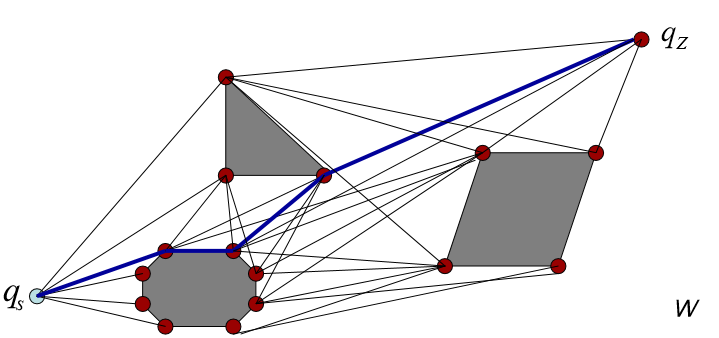
\includegraphics[width=12cm]{BilderInke/Sichtbarkeitsgraph.png}
	\caption{Beispiel Sichtbarkeitsgraph, Graue Felder sind Hindernisse, blaue Linie ist optimaler Pfad}
	\label{fig:Sichtbarkeitsgraph}
	\cite{WegPlanung}
\end{figure}

Durch Einsatz der A*-Methode kann so der optimale Pfad bestimmt werden. Die Kanten zwischen zwei Knotenpunkten werden von dem Algorithmus je nach Anforderung, beispielsweise k�rzester Weg, gewichtet. Je gr��er diese Gewichtung ist, desto weiter Weg befindet sich der Knotenpunkt am anderen Ende der Kante. Die direkte Entfernung eines Knotenpunktes zum Zielpunkt wird gesch�tzt, so dass die Knoten ebenfalls eine Gewichtung bekommen. 

Vom Zielpunkt aus werden nun alle Knoten betrachtet, die �ber eine Kante erreicht werden k�nnen. Der aus der Betrachtung hervorgehende Knotenpunkt, der die geringste direkte Entfernung zum Ziel aufweist, wird als n�chstes untersucht. Die anderen werden gespeichert und im weiteren Verlauf mit Konten hinsichtlich ihrer Gewichtung verglichen. Punkte, die bereits betrachtet wurden, werden  als \glqq untersucht \grqq{} markiert. Dieses Verfahren wiederholt sich so lange bis der optimale Pfad gefunden wurde. Ein solcher Pfad ist in der obenstehenden Abbildung als dicke blaue Linie dargestellt. 

Ein Vorteil dieser Methode ist, dass immer der optimale Pfad vom Start zum Ziel gefunden wird. Nachteile sind jedoch, dass der Pfad immer direkt an den Ecken und Kanten der Hindernisse entlang f�hrt. Au�erdem kann bei vielen Hindernissen, beispielsweise Hindernisse mit vielen Ecken und Kanten, ein sehr gro�er Graph entstehen, der viel Rechenzeit in Anspruch nimmt. 

\subsubsection{Occupancy Grid mit D*-Algorithmus}
Wie der Name \glqq Occupancy Grid\grqq{} vermuten l�sst, wird der Raum in ein Gitternetz unterteilt. Jede entstehende Zelle kann mit einer \glqq 1\grqq{} f�r \glqq belegt\grqq{} und \glqq 0\grqq{} f�r \glqq frei\grqq{} versehen werden. Dadurch entsteht eine Umgebungskarte, in der Hindernisse und freier Raum zum Fahren klar definiert sind. In der Abbildung \ref{fig:OccupancyGrid} ist ein Beispiel des Occupancy Grids dargestellt. Dabei sind anstatt Zahlen in den Zellen die freien Bereiche wei� und die besetzten Bereiche rot dargestellt. Der �bersichtlichkeit halber ist ein gr��eres Gitternetz dargestellt, als eigentlich unterteilt.\cite{Robotics}\\

\begin{figure}[H]
	\centering	
	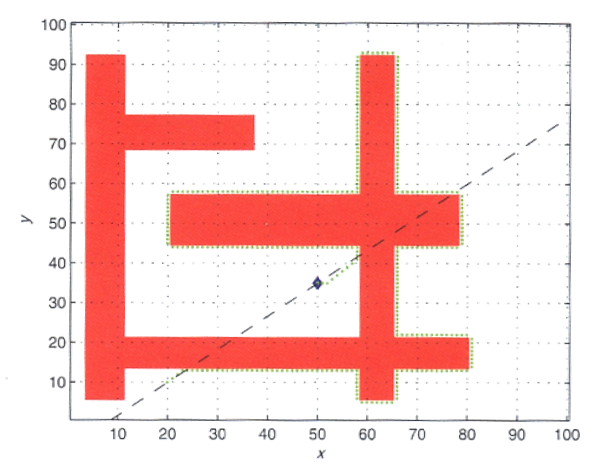
\includegraphics[width=10cm]{BilderInke/OccupancyGrid.png}
	\caption{Beispiel Occupancy Grid, Rot-Hindernisse, Wei�-befahrbarer Raum}
	\label{fig:OccupancyGrid}
	\cite{Robotics}
\end{figure}

Der D*-Algorithmus ver�ndert die Bewertung der einzelnen Zellen mit einem neuen Wert, der die \glqq Kosten\grqq der Zelle repr�sentiert. Zellen, die zu einem Hindernis geh�ren werden mit \glqq $ \infty $\grqq gewichtet. Je h�her die Gewichtung ist, desto weiter weg befindet sich das Ziel. Mit diesem Algorithmus wird immer der optimale Pfad gefunden. Je nach Aufgabenstellung kann diese Gewichtung zum Beispiel Distanz oder Zeit bedeuten. 
In der nachstehenden Abbildung \ref{fig:Occupancy Grid mit D*-Algorithmus} ist der geplante Weg von dem Startpunkt zum Ziel mittels gr�n gepunkteter Linie dargestellt. Die Hindernisse sind rot markiert. Die Intensit�t des Grautons im Hintergrund gibt in diesem Fall die Entfernung zum Ziel an. 
\begin{figure}[H]
	\centering	
	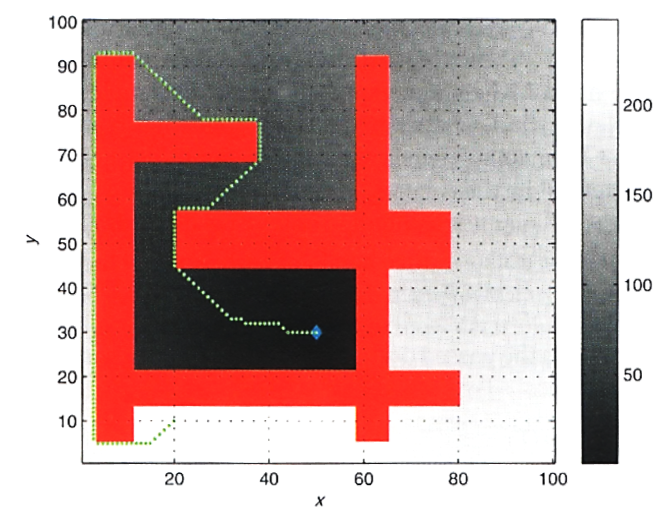
\includegraphics[width=10cm]{BilderInke/DStern.png}
	\caption{Beispiel Occupancy Grid mit D*, Rot-Hindernisse, Intensit�t des Graus im Hintergrunds repr�sentiert die Entfernung zum Ziel; blauer Punkt entspricht Ziel}
	\label{fig:Occupancy Grid mit D*-Algorithmus}
	\cite{Robotics}
\end{figure}

Ein Vorteil dieser Methode ist, dass der Weg schrittweise neu geplant werden kann. Sollte der Raum anders sein, als zuvor in dem Gitternetz eingetragen, eine Zelle beispielsweise teurer sein als geplant, so kann stufenweise ein besserer Pfad gefunden werden. Die Berechnung des neuen Weges erfordert nicht so viel Rechenleistung, wie eine komplett neue Wegplanung, da nur die Zellen in direkter Umgebung betrachtet werden. Die Anfangsberechnung ist hingegen sehr rechenintensiv. Zudem ben�tigt das Occupancy Grid bei hoher Aufl�sung viel Speicherplatz.

\subsection{Lokale Bahnplanung}
Die lokale Bahnplanung betrachtet nur das direkte Umfeld des Roboters. Lokale Bahnplanungsalgorithmen planen den Weg zum Ziel weniger vorausschauend. Daher ben�tigen sie in der Regel weniger Rechenzeit und sind somit schneller als globale Bahnplanungsmethoden. Mit den aktuellen Umgebungsdaten und Sensorinformationen wird ein lokales Navigationsziel angestrebt. Ziel ist hierbei die reaktive Kollisionsvermeidung. 
Im Folgenden werden zwei M�glichkeiten den lokalen Bahnplanung beschrieben: 
\begin{itemize}
\item \textbf{Bug-Algorithmus}
\item \textbf{Potentialfeld-Methode}
\end{itemize}

\subsubsection{Bug-Algorithmus}
Der \glqq Bug-Algorithmus \grqq{} ist im Allgemeinen eine reaktive Navigationsmethode und basiert auf dem Prinzip, dass sich der Roboter so lange entlang eines Hindernisses bewegt, bis er wieder freie Fahrt in Richtung Ziel hat. Es gibt verschiedene Algorithmen, die diese Methode verfolgen. Dazu geh�rt der \glqq Bug1 -\grqq, \glqq Bug2-\grqq, \glqq Bug3-\grqq und \glqq DistBug-Algorithmus \grqq{}. Im Folgenden wird nur der Bug2-Algorithmus n�hergehend erl�utert. \cite{Bug2} \cite{WegPlanung} 

Unter Verwendung des betrachteten Algorithmus kennt der Roboter zu jeder Zeit den direkten Weg zwischen seiner Startposition und dem Ziel. Hierbei werden m�gliche Hindernisse zun�chst nicht ber�cksichtigt. Abgesehen von einem Ziel im globalen Raum, kennt der Roboter nur seine direkte Umgebung. Der direkte Weg wird hier m-Linie genannt. Ein Beispiel ist in der untenstehenden Abbildung \ref{fig:Bug2_m-Linie} dargestellt.

\begin{figure}[H]
	\centering	
	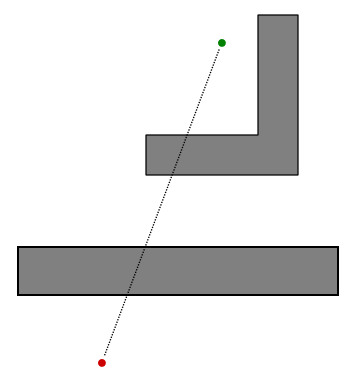
\includegraphics[width=5cm]{BilderInke/Bug2_m-Linie.png}
	\caption{Bu2-Algorithmus, Grauen Fl�chen: Hindernisse, Roter Punkt: Startpunkt, Gr�ner Punkt: Ziel, Verbindungslinie: m-Linie}
	\label{fig:Bug2_m-Linie}
	\cite{Bug2}
\end{figure}
Der rote Punkt in der Abbildung ist die Startposition und der gr�ne das Ziel. 
Die Anweisung des Algorithmus an den Roboter k�nnen in drei einfache Befehle unterteilt werden. 

\begin{itemize}
\item \textsl{Fahre auf der m-Linie Richtung Ziel}
\item \textsl{Ist ein Hindernis im Weg, dann fahre an dessen Kante entlang, bis die  m-Linie wieder erreicht wird}
\item \textsl{Ist die m-Linie wieder erreicht, verlasse das Hindernis und fahre weiter Richtung Ziel}
\end{itemize}

Wie ein m�glicher Weg des Roboters unter dem Bug2-Algorithmus aussehen k�nnte, ist in Abbildung \ref{fig:Bug2} zusehen. Die orangene Linie zeigt dabei den Fahrweg des Roboters

\begin{figure}[H]
	\centering	
	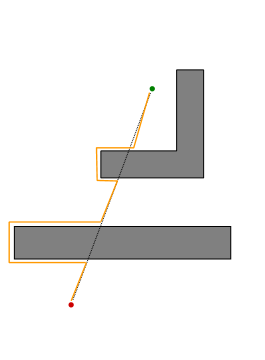
\includegraphics[width=5cm]{BilderInke/Bug2.png}
	\caption{Bu2-Algorithmus, Fahrweg des Roboters ist in orange dargestellt}
	\label{fig:Bug2}
	\cite{Bug2}
\end{figure}

Der Bug2-Algorithmus ist ein vergleichsweise einfacher Algorithmus. Das Entlangfahren an den Hindernissen kann nur in eine Richtung, links oder rechts, vorgegeben werden. Somit ist nicht garantiert, dass immer der optimale Pfad gefunden wird. Au�erdem kann es zu einer Art \glqq Deadlock\grqq{} kommen, wenn der Roboter an einer Kante des Hindernissen entlang fahren muss, die m-Linie jedoch nicht wieder findet. Ein solches Szenario ist in Abbildung \ref{fig:Bug2_Problem} dargestellt. 

\begin{figure}[H]
	\centering	
	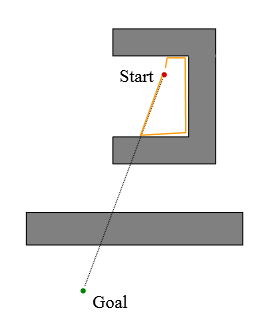
\includegraphics[width=5cm]{BilderInke/Bug2_Problem.png}
	\caption{Bu2-Algorithmus, m�glicher Deadlock,  Fahrweg des Roboters ist in orange dargestellt}
	\label{fig:Bug2_Problem}
	\cite{Bug2}
\end{figure}

\subsubsection{Potentialfeld-Methode}
Bei der Potentailfeld-Methode ist der Roboter k�nstlichen Kr�ften von Zielen und Hindernissen ausgesetzt. Die hohen Potentiale sto�en den Roboter ab, niedrigere Potentiale ziehen ihn an. Jeder Punkt in dem Konfigurationsraum erh�lt ein Potential. So wird dem Start ein hohes und dem Ziel ein sehr niedriges Potential zugeordnet. Hindernisse bekommen sehr hohe Potentiale. Die Bewegungsrichtung des Roboters kann �ber die Gradientenberechnung des Potentialfeldes erfolgen, da der Roboter auf seinem Weg vom Start zum Ziel dem negativen Gradienten des globalen Potentialfeldes folgt. In die Berechnung des Gradienten gehen nur die Hindernisse mit ein, die sich in relativer N�he zum Roboter befinden.\cite{WegPlanung} In der Abbildung \ref{fig:Potentialfeld} ist ein Beispiel eines Potentialfeldes dargestellt. Das niedrige Potential des Ziels ist in blau dargestellt. 

\begin{figure}[H]
	\centering	
	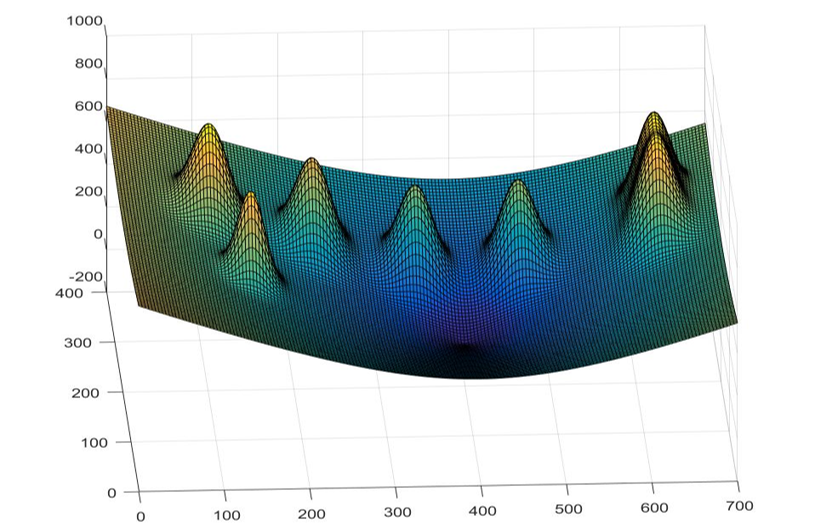
\includegraphics[width=15cm]{BilderInke/Potentialfeld.png}
	\caption{Beispiel Potentialfeld}
	\label{fig:Potentialfeld}
\end{figure}

Die Vorteile der Potentialfeld-Methode sind sowohl die einfache Implementierung als auch die geringe Rechenzeit. Durch die Echtzeit-Kollisionsvermeidung ist das System sehr dynamisch. Es besteht jedoch die Gefahr, dass lokale Minima entstehen, aus denen der Robotino nicht wieder raus kommt.  

\section{Ausgew�hltes Konzept}

An der zu simulierenden Produktionsstra�e sind bis zu f�nf Robotinos gleichzeitig beteiligt. Um einen zuverl�ssigen Produktionsablauf sicherstellen zu k�nnen, werden hohe Anforderungen an die Bahnplanungsmethode gestellt. Die Methode muss dynamisch und zuverl�ssig sein und sollte geringen Rechenaufwand ben�tigen. Die soeben erl�uterten Methoden sind in der Tabelle \ref{tab: Methodenvergleich}, reduziert auf die wichtigsten Eigenschaften, �bersichtliche dargestellt. 

\begin{table}[H]
\caption{Bahnplanungsmethoden nach ihrer Dynamik, Sicherheit, Rechenzeit und Zuverl�ssigkeit bewertet}
 \begin{tabular}{lcccc}
 
  Methode & Dynamik & Sicherheit & Rechenzeit & Zuverl�ssigkeit \\
  \hline 
  Sichtbarkeitsgraph mit A* & gering & mittel & mittel/hoch & sehr hoch \\
  Occupancy Grid mit D* & mittel & hoch & mittel/hoch & hoch \\
  Bug-Methode & mittel & gering & gering & gering \\
  Potentialfeld-Methode & sehr hoch & mittel & gering & hoch \\
  
  \label{tab: Methodenvergleich}
  
 \end{tabular}
\end{table}
Bei sehr hoher Dynamik und hoher Zuverl�ssigkeit ben�tigt die Potentialfeld-Methode nur wenig Rechenzeit. Damit ist sie von den betrachteten Methoden die beste. Das Potentialfeld hat zudem den Vorteil, dass ein komplett autonomes Gesamtsystem geschaffen werden kann, da es f�r die Trajektorienberechnung nicht notwendig ist das Ziel und die Fahrtroute der anderen Robotinos zu kennen. 

\subsection{Gesamtkonzept}

Im Folgenden wird das Gesamtkonzept mit der Bahnplanungsmethode Potentialfeld kurz erl�utert. Genauere Erkl�rungen mit Ausz�gen aus dem Originalprogramm werden anschlie�end erl�utert. 
\begin{figure}[H]
	\centering	
	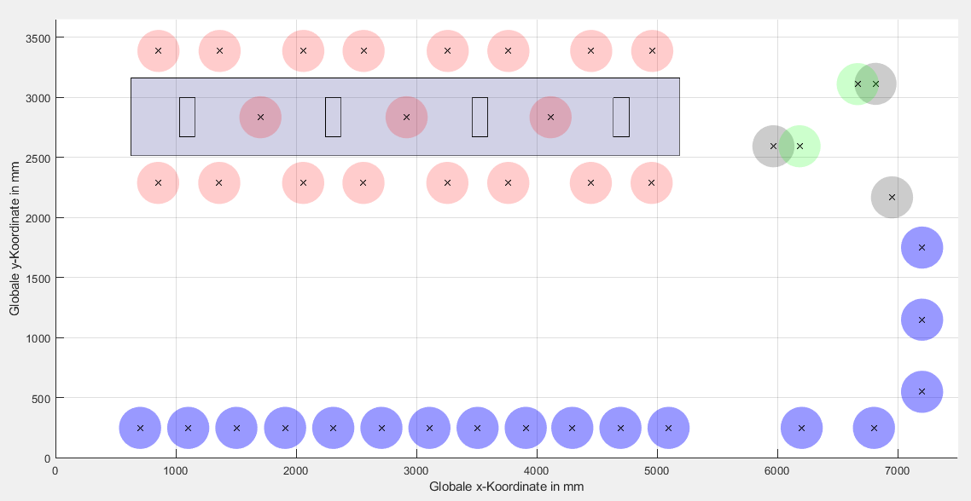
\includegraphics[width=14cm]{BilderInke/KonfigRaum.png}
	\caption{Konfigurationsraum mit Wartepositionen, Fifo-Positionen, Stationen und �bergabepunkten}
	\label{fig:Konfigurationsraum}
\end{figure}
Der Konfigurationsraum ist in Abbildung \ref{fig:Konfigurationsraum} mit globalem Koordinatensystem, eingezeichneten Stationen, Wartepositionen und �bergabepunkten dargestellt. 

\subsubsection{Wartepositionen}
\label{Wartepositionen}
Jedem Robotino wird eine eigene Warteposition am Rand des Konfigurationsraumes zugeordnet. Diese Warteposition ist zu Beginn des Gesamtsystem die Startposition des jeweiligen Robotinos und immer dann Zielposition, wenn der Robotino keinen Auftrag empf�ngt. Sollten alle \glqq Fifo-Pl�tz\grqq{} (vgl. Kapitel \ref{Warteschlange}) einer Station belegt sein, so dass sich ein Robotino nicht mehr anstellen kann, muss er auf seiner Warteposition auf einen freien Platz warten. 

\subsubsection{Stationen und �bergabepunkte}
\label{Stationen und �bergabepunkte}
Wie in Abbildung \ref{fig:Konfigurationsraum} zu sehen ist, befindet sich vor und hinter jeder Station �bergabepunkte. Hat ein Robotino die Aufgabe zu einer Station zu fahren, f�hrt er stattdessen nur vor die Station auf den �bergabepunkt. Ab da wird die Steuerung des Roboters an das Gewerk3 \glqq Regelung\grqq{} �bergeben. Sollten mehrere Robotinos die gleiche Station anfahren wollen, so darf der Robotino die Station zuerst befahren, der den �bergabepunkt zuerst erreicht hat. �ber die �bergabepunkte wird die Station auch wieder verlassen. Der vordere �bergabepunkt wird immer dann genutzt, wenn sich kein weitere Robotino im Fifo befindet. �ber den hinteren �bergabepunkt wird die Station verlassen, wenn ein andere Robotino bereits im Fifo (vgl. Kapitel \ref{Warteschlange}) wartet. 
Das Potentialfeld ist in den Stationen, solange Gewerk3 \glqq Regelung\grqq{} den Robotino steuert, nicht aktiv. Aktiviert beziehungsweise ausgeschaltet wird das Potentialfeld zum Zeitpunkt der �bergabe. Sollte ein Robotino, aufgrund eines notwendigen Ausweichman�vers, in eine Station gedr�ckt werden, so verl�sst er sie unverz�glich nach hinten raus. In diesem Fall bleibt das Potentialfeld aktiv. 

\subsubsection{Warteschlange \glqq Fifo\grqq}
\label{Warteschlange}
Ist eine Station, in die ein Robotino fahren soll, bereits belegt, so f�hrt er zu der zugeh�rigen Warteschlange, dem sogenannten \glqq Fifos\grqq{}. Die Fifos, die sich am Rand des Konfigurationsraumes befinden, sind Wartepositionen f�r die Stationen, um w�hrend des Wartens den befahrbaren Raum nicht zu blockieren. Der Robotino, der die Warteschlange zuerst betreten hat, darf diese, sobald die Station wieder frei ist, auch als erster wieder verlassen. Erst, wenn dieser die Station erreicht hat, r�cken eventuell wartende Robotinos im gleichen Fifo auf. 

\subsubsection{Ladestation}
\label{Ladestation}
Die Ladestationen befinden sich an der rechten Seite des Konfigurationsraumes. Eine Ladestation ist f�r die Robotinos 1.0 und eine weitere f�r den Robotino 2.0. Auch hier sind �bergabepunkte definiert. Aus platztechnischen Gr�nden muss der Robotino 2.0 von hinten an die Ladestation fahren. Um dieses m�glichst effizient zu realisieren, ist der �bergabepunkt f�r diese Ladestation vergleichsweise weit im eigentlichen Transportbereich. Ab diesem Punkt wird an Gewerk3 �bergeben, welches den Robotino 2.0 mittels hoch genauer Regelung vor und in die Ladestation fahren l�sst. 

\subsubsection{Potentialfeld}
\label{Potentialfeld}
Hindernisse im Potentialfeld werden mit hohen Potentialen versehen. Zu diesen Hindernissen geh�ren hier die Stationen und die Robotinos. In Abbildung \ref{fig:Potentialfeld-Fertig} ist das gesamte Potentialfeld dargestellt, das auf jeden Robotino geladen wird. 
\begin{figure}[h!]
	\centering	
	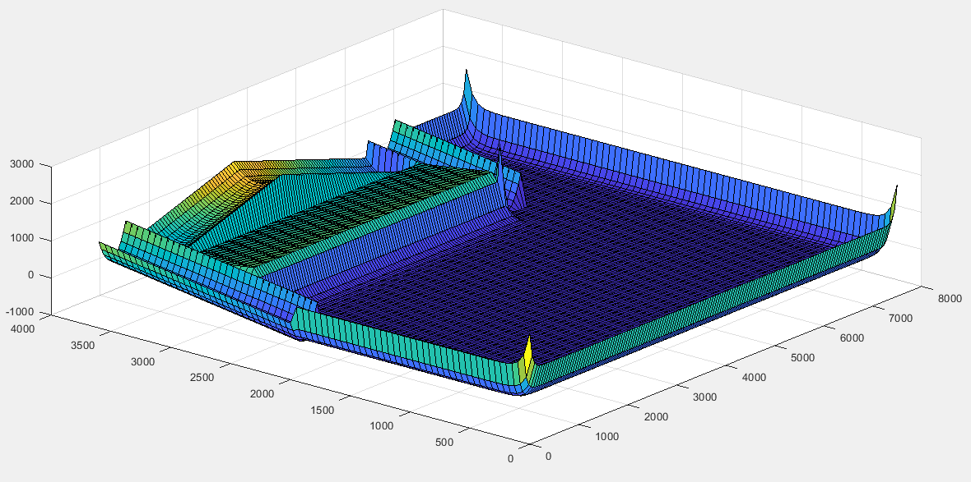
\includegraphics[width=15cm]{BilderInke/Potentialfeld_Fertig.png}
	\caption{Potentialfeld des Konfigurationsraumes eingez�unt in hohe Potentiale zur eindeutigen Begrenzung des Raumes, Stationen als ein hohes Potential dargestellt, Rampen und Fahrrinnen zum leiten der Robotinos, }
	\label{fig:Potentialfeld-Fertig}
\end{figure}

�ber eine Begrenzung durch hohes Potential wird der Raum, in dem sich die Robotinos bewegen d�rfen, eindeutig definiert. Die Stationen sind als ein gesamter Block mit hohem Potential dargestellt, da der Robotino zu keiner Zeit zwischen oder an eine Station fahren soll, wenn nicht zuvor die �bergabe an Gewerk3 erfolgt ist. 
Zur Vermeidung von kritischen Situationen oder lokalen Minima zwischen Stationen und Wand sind Rampen und Fahrrinnen implementiert, die je nach Station den Roboter nach links oder rechts in eine Fahrrinne und von dort in den frei befahrbaren Raum f�hren. 

%\chapter{Konzept}
\chapter{Konzept}
In diesem Kapitel wird das in diesem Bericht genutzte Konzept beschrieben. Das Grundkonzept bestehet darin, dass der zu befahrene Bereich in einen Fertigungsbereich und einen Transportbereich unterteilt wird. Die Grenzen der Bereiche sind in Abbildung \ref{fig:Bereiche} dargestellt. Im Transportbereich, in der Abbildung \ref{fig:Bereich} nicht eingefärbt, wird die Regelung des Robotinos über die Potentialfeldmethode realisiert. Das dabei genutzte Potentialfeld wird unter Kapitel \ref{sec:Potential} näher erläutert. Im Fertigungsbereich wird die Regelung von der Bahnregelungsgruppe übernommen. Um zwischen den Bereichen zu wechseln, werden Übergabepunkte definiert, an denen der Bereichswechsel sicher ausgeführt werden kann. Diese Übergabepunkte sind in der Abbildung als rote Kreise dargestellt. Dazu wird eine Kommunikation zwischen den Einzelgruppen über eine Schnittstelle definiert. Diese Schnittstelle wird in Kapitel \ref{} definiert. Desweiteren wird das Konzept zum Vermeiden von Kollisionen in Kapitel \ref{} näher beschrieben. Dabei wird auf verschiedene Hindernistypen eingegangen. Um das Konzept abzuschließen wird in Kapitel \ref{} der Ablauf des Programmes dargestellt.

\begin{figure}[!h]
	\centering	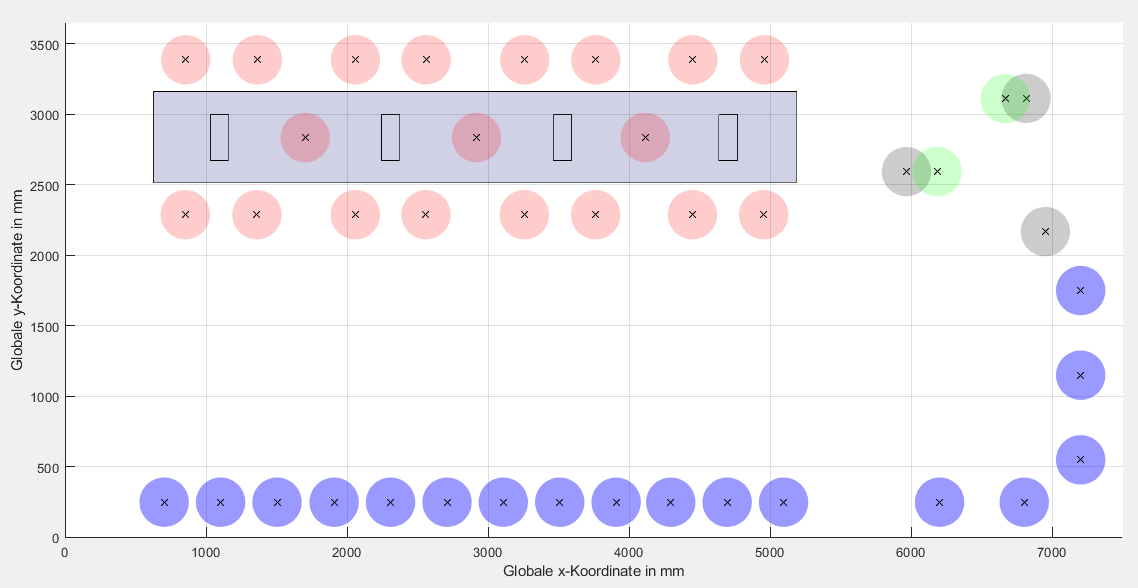
\includegraphics[width=0.8\textwidth]{grafiken/TransportbereichKarte.png}
	\caption{Bereichseinteilung}
	\label{fig:Bereiche}
\end{figure}
%\section{Potentialfeld zur Bahngenerierung und Kollisionsvermeidung}
\section{Potentialfeld zur Bahngenerierung und Kollisionsvermeidung}
\label{sec:Potential}
In diesem Abschnitt wird beschrieben, wie das Potentialfeld aufgebaut ist, das zur Generierung des Geschwindigkeitsvektors genutzt wird.
\subsection{Roboter Umwelt}
Um die statische Umwelt des Robotinos im Potentialfeld darzustellen, wird der zu befahrende Bereich in Zonen unterteilt. Die gew�hlten Zonen sind in Abbildung \ref{fig:PotZonen} farbig dargestellt. In Tabelle \ref{tab:Zonen} ist die Zuordnung der Zonen zur Abbildung \ref{fig:PotZonen} beschrieben. Dabei wird eine Hauptfahrzone (Zone 0) definiert, in der mit einem virtuellen Zaun der zu befahrene Bereich abgegrenzt wird. Dieser Zaun ist notwendig, damit die Zone nicht unkontrolliert verlassen wird, dazu werden e-Funktionen genutzt, die in den Funktionen \eqref{fun:H01} bis \eqref{fun:H03} definiert sind. Aufgrund der Form der Zone m�ssen dabei drei Funktionen definiert werden, die je nach Position des Robotinos ausgef�hrt werden. Das Verlassen der Zone 0 erfolgt durch die �bergabe an den Fertigungsbereich, welches in Kapitel \ref{sec:Kon_Bahnregelung} n�her erl�utert wird. \\
Zone 1 bis 3 dienen zur R�ckf�hrung der Robotinos zur Zone 0, dazu wird ein Potentialfeld genutzt, dass uns erm�glicht den Robotino in eine gezielte Richtung zu lenken. Die dazu genutzten Funktionen sind unter \eqref{fun:H1} bis \eqref{fun:H3} definiert. Diese Potentialfelder nutzen in Fahrrichtung eine Geradengleichung mit definierter Steigung und senkrecht dazu eine Parabelform, um den Robotino auf Kurs zu halten. Wenn sich der Robotino in Zone 4 befindet, wird dieser �ber eine Geradengleichung nach hinten gef�hrt. Die dabei genutzte Gleichung ist als \eqref{fun:H4} gekennzeichnet. Zus�tzlich wird in Zone 4 f�r jede Station eine gau�sche radiale Basisfunktion, welche unter Kapitel \ref{sec:PotRob} n�her erl�utert, genutzt, damit keine Kollision mit den Stationen auftreten. Diese Zone wird nur im Fehlerfall oder beim Start des Robotinos betreten, da in dieser Zone der Fertigungsbereich aktiv ist. Die Zone 5 dient dazu den Robotino gezielt in Richtung der Mitte der Zone 0 zu f�hren. Dazu wird, wie in Zone 1 bis 3, eine Parabel mit einer Geradengleichung genutzt. Die dabei genutzte Funktion ist als \eqref{fun:H5} definiert. Dabei ist zu beachten, dass vorgesehen ist, dass Zone 5 nur aktiv ist, wenn sie aus Zone 1 betreten wird. Dadurch wird die Anfahrm�glichkeit aus der Zone 0 zur Ladestation gew�hrleistet. \\
Je nach Zone gilt dabei ein eigenes Potentialfeld, welche kombiniert das Gesamtpotentialfeld ergebenen. Die einzelnen Zonen sind in Abbildung \ref{fig:Poteinzeln} dargestellt. Das gesamt Potentialfeld ist in Abbildung \ref{fig:PotUmweltohne} dargestellt, wobei zur �bersichtlichkeit die Stations und Ladestationspotentiale nicht dargestellt werden. Da die Zone 5 nur durchlaufen wird, wenn sie aus Zone 1 betreten wird, wird in Abbildung \ref{fig:PotUmweltmit} dargestellt, wie das Potentialfeld in diesem Fall aussieht.

\begin{table}
\centering
 \begin{tabular}{|c|c|c|}
  \hline Zone & Farbe & Beschreibung \\ 
  \hline 0 & ohne Farbe & Hauptfahrzone \\
  \hline 1 & Gr�n &  F�hrung des Robotinos nach Zone 5 \\
  \hline 2 & Blau &  F�hrung des Robotinos nach Zone 3 \\
  \hline 3 & Violet & F�hrung des Robotinos nach Zone 0 \\
  \hline 4 & Rot & F�hrung des Robotinos nach Zone 1 und 2\\
  \hline 5 & Cyan & F�hrung des Robotinos nach Zone 0 \\
   \hline \end{tabular}
   \caption{Zuordnung der Farben aus Abbildung \ref{fig:PotZonen}}
   \label{tab:Zonen}
\end{table}

\begin{figure}
	\centering	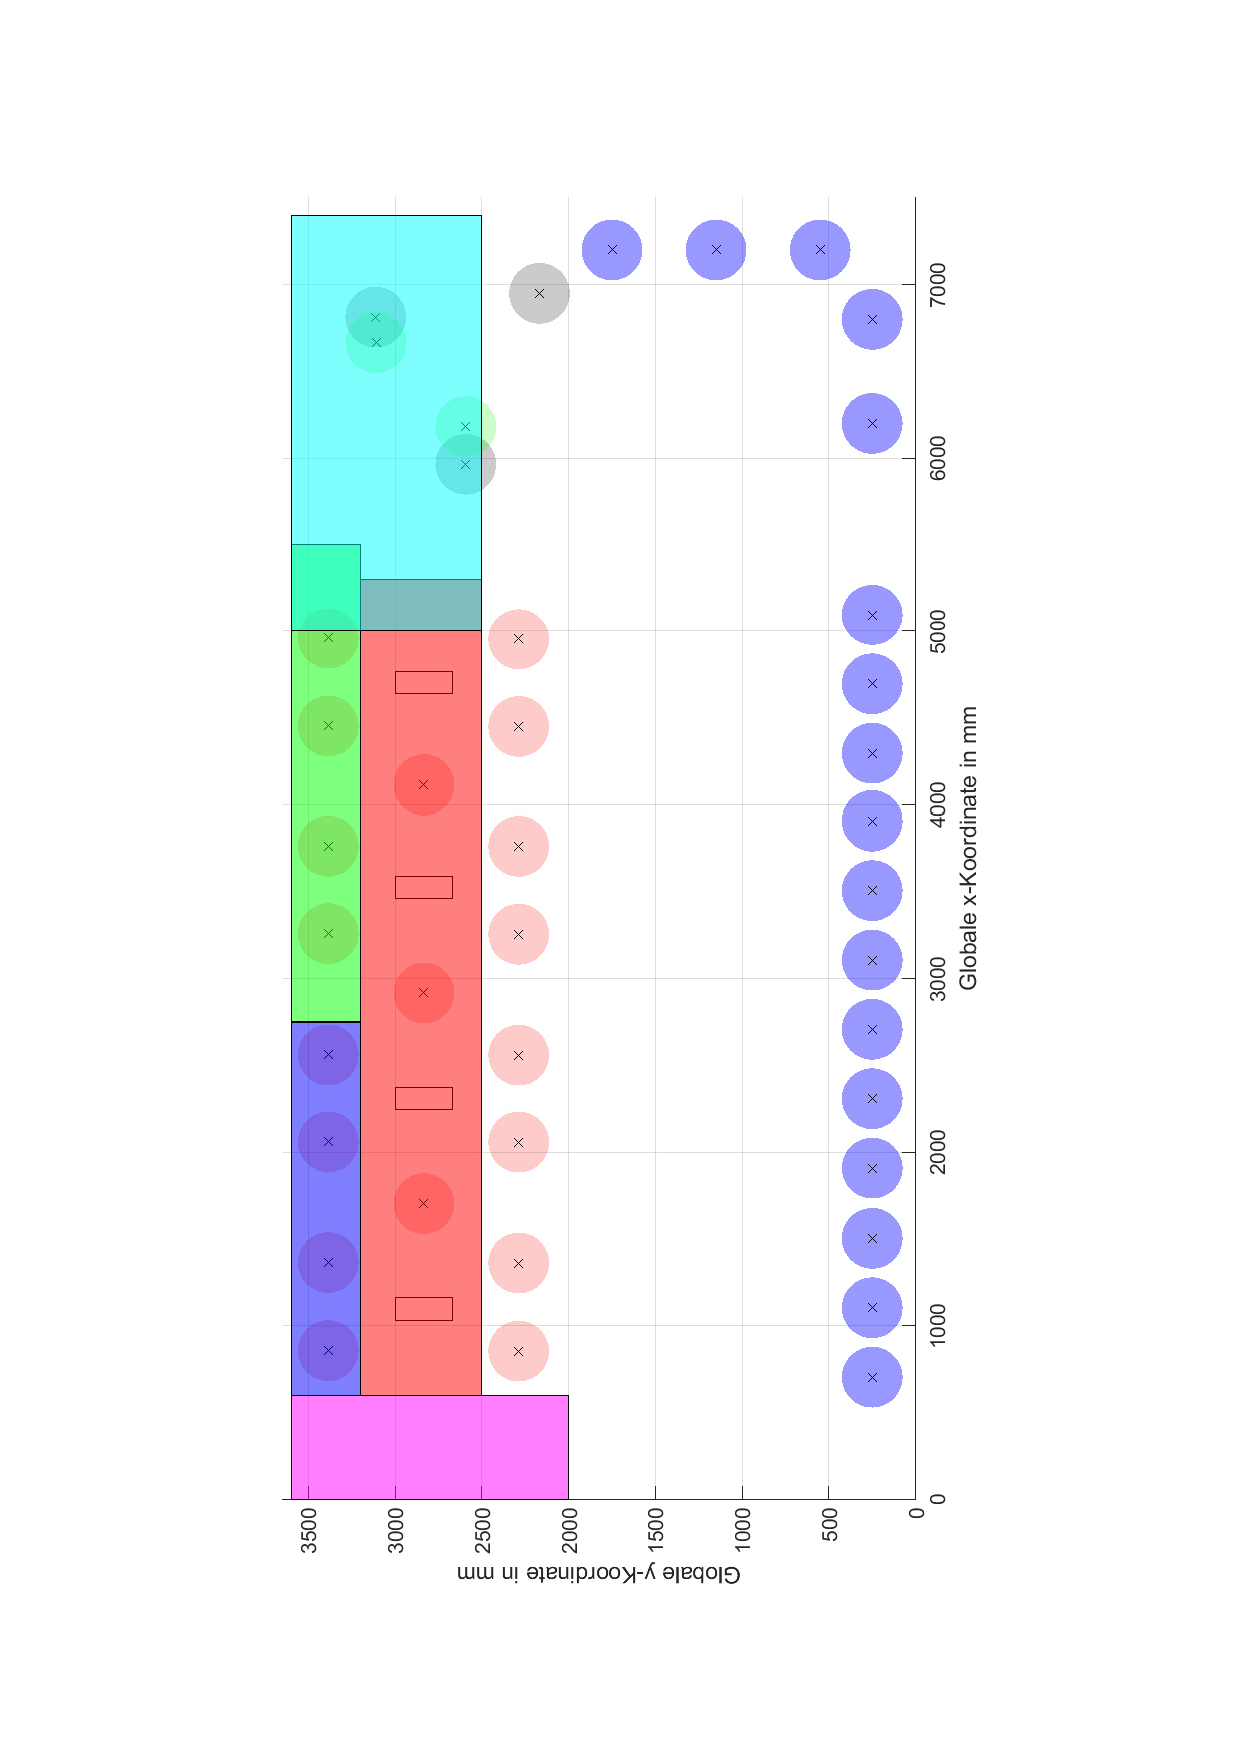
\includegraphics[width=0.8\textwidth, angle=-90]{grafiken/Zonen_eingezeichnet.pdf}
	\caption{Potentialfeldzonen}
	\label{fig:PotZonen}
\end{figure}

\scalebox{0.8}{\begin{minipage}{1.2\textwidth}
\begin{align}
\label{fun:H01}
H_{0(x=0..5500,y=0..2500)}(x,y)= K_{exp}\cdot(e^{(-\frac{x}{\sigma})}+e^{(\frac{x-7400}{\sigma})}+e^{(-\frac{y}{\sigma})}+e^{(\frac{y-2500}{\sigma})} ) \label{fun:H01}\\ 
\label{fun:H02}
H_{0(x=5500..7400,y=0..2500)}(x,y) = K_{exp}\cdot(e^{(-\frac{(x-5500)-(y-2500)}{\sigma})}+e^{(\frac{x-7400}{\sigma})}+e^{(-\frac{y}{\sigma})} )\\ 
\label{fun:H03}
H_{0(x=5500..7400,y=2500..3600)}(x,y) = K_{exp}\cdot(e^{(-\frac{(x-5500)}{\sigma})}+e^{(\frac{(y-3600)}{\sigma})}+e^{(\frac{x-7400}{\sigma})}+e^{(-\frac{y}{\sigma})} )\\ 
\label{fun:H1}
H_{1}(x,y) = - K_{gerade}\cdot x + K_{parabel}\cdot\frac{(y-3500)^2}{B}\\
\label{fun:H2}
H_{2}(x,y) = K_{gerade}\cdot x + K_{parabel}\cdot\frac{(y-3500)^2}{B}\\
\label{fun:H3}
H_{3}(x,y) = K_{parabel}\cdot\frac{(x-300)^2}{B} + K_{gerade}\cdot y\\
\label{fun:H4}
H_{4}(x,y) = - K_{gerade}\cdot y\\
\label{fun:H5}
H_{5}(x,y) = K_{parabel}\cdot\frac{(x-5500)^2}{B}-K_{gerade}\cdot y
 \end{align}
\end{minipage}}

\begin{figure}
	\centering	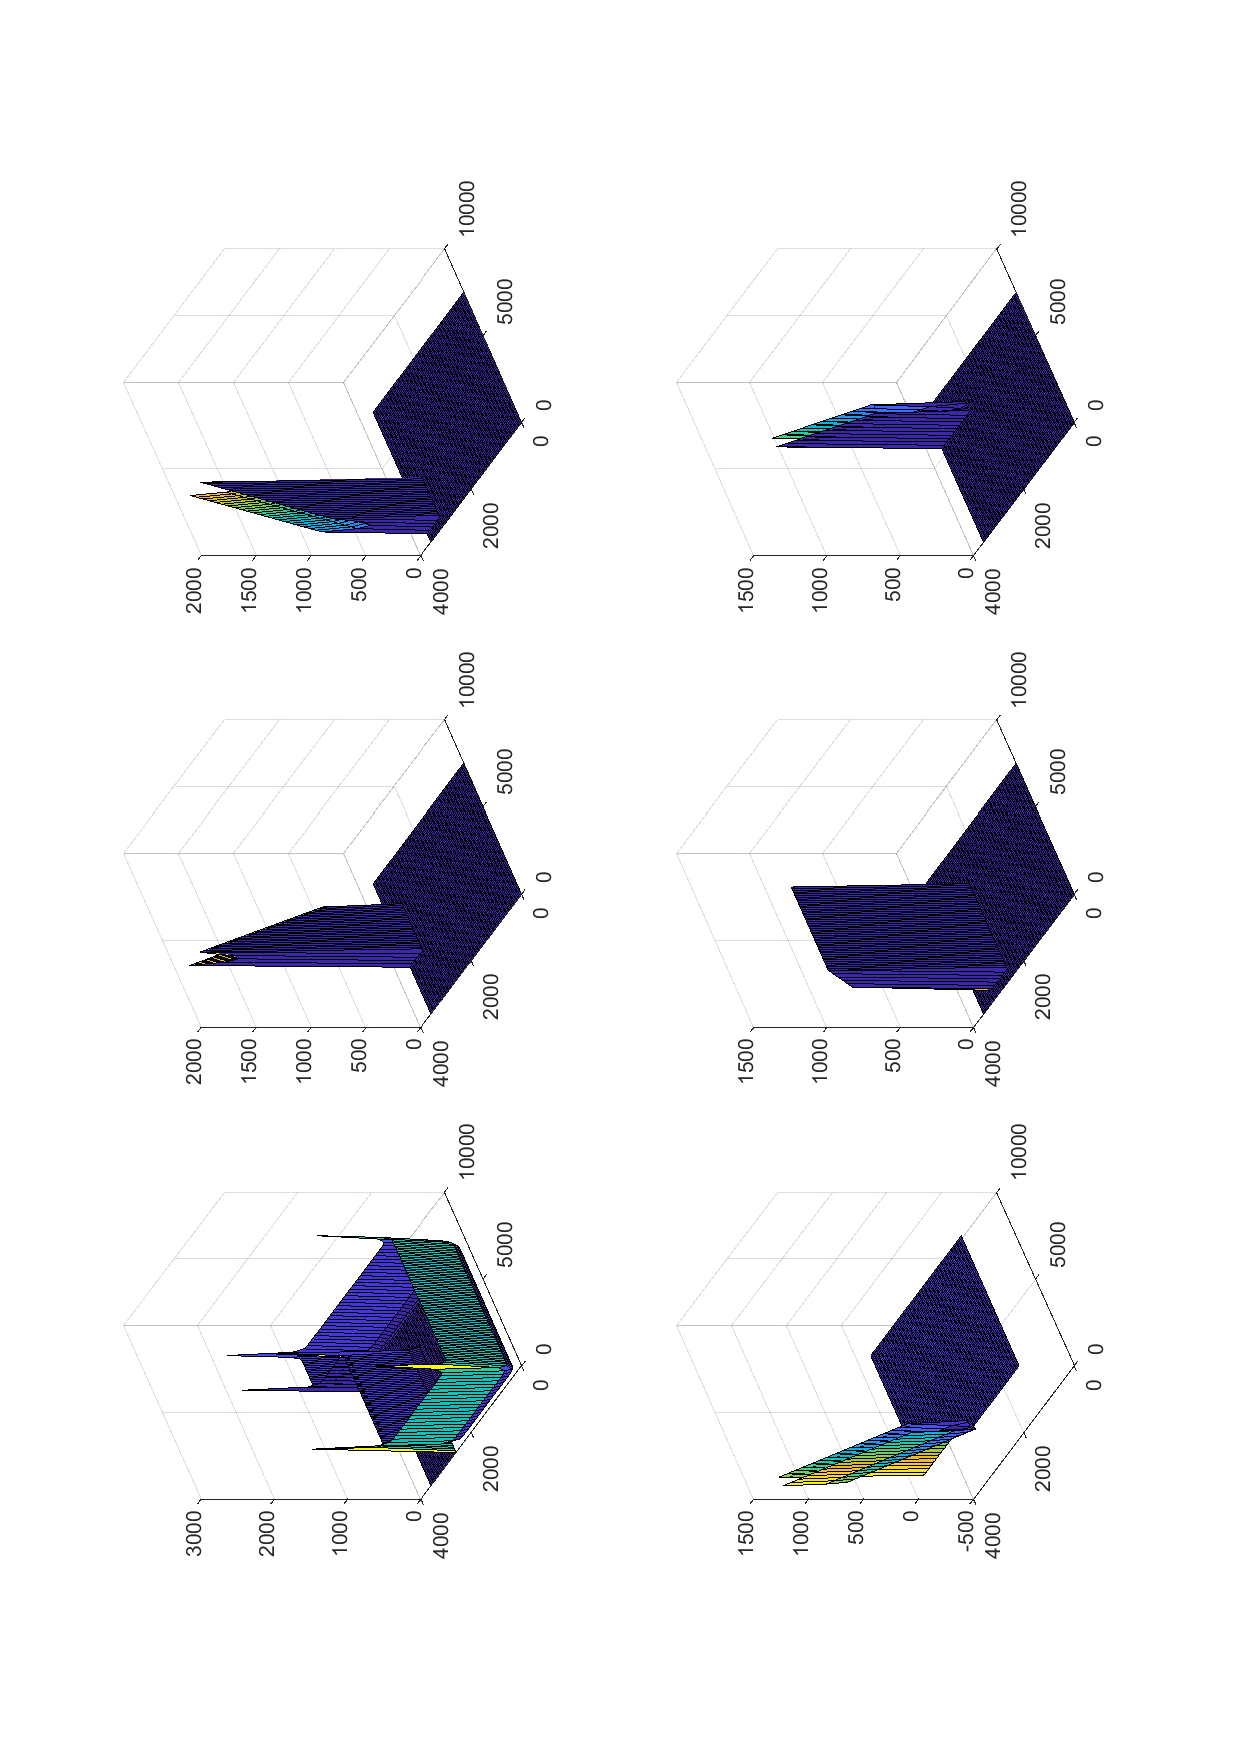
\includegraphics[width=0.8\textwidth,angle=-90]{grafiken/EinzelZonen.pdf}
	\caption{Potentialfeld der einzel Zonen}
	\label{fig:Poteinzeln}
\end{figure}

\begin{figure}
	\centering	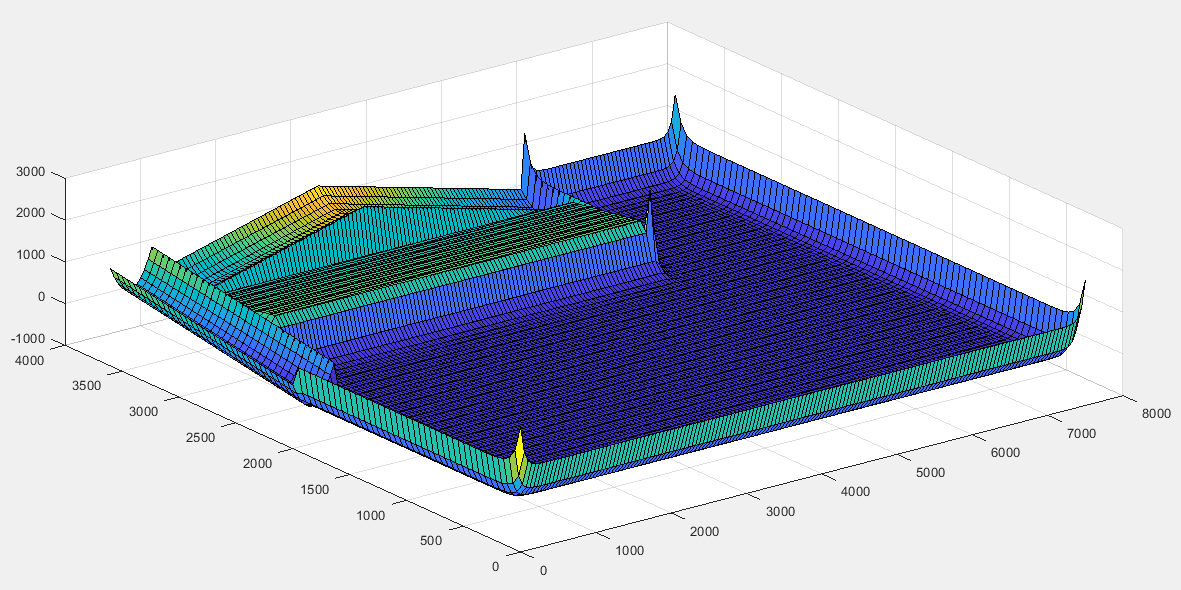
\includegraphics[width=0.8\textwidth]{grafiken/Potentialfeld_ohne_2schraege.png}
	\caption{Potentialfeld der Roboter Umwelt ohne Rausf�hrung}
	\label{fig:PotUmweltohne}
\end{figure}

\begin{figure}
	\centering	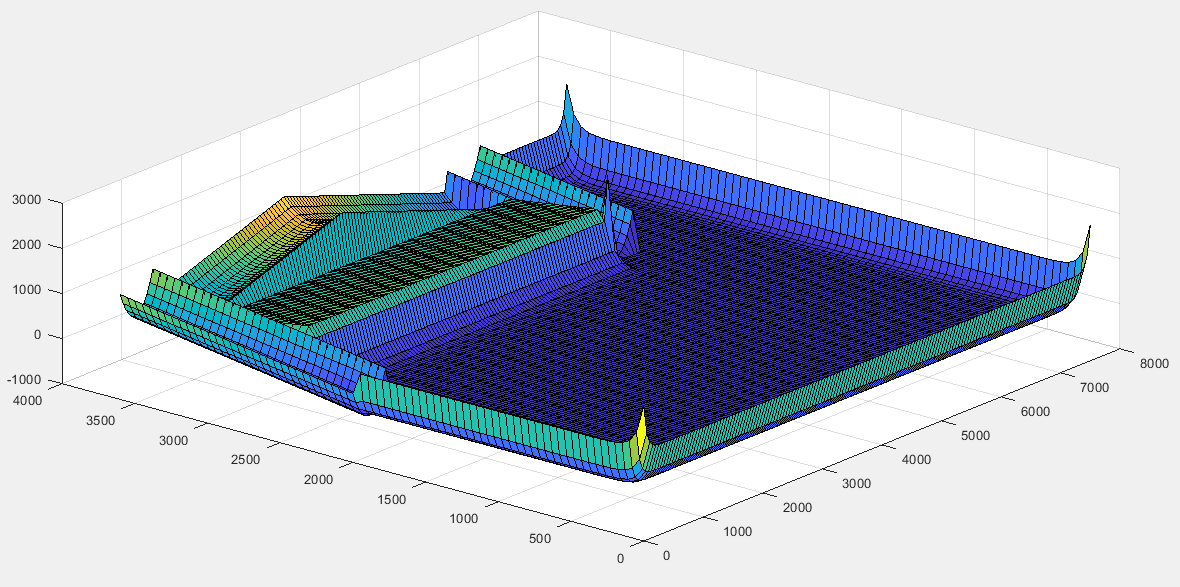
\includegraphics[width=0.8\textwidth]{grafiken/Potentialfeld_mit_2schraegen.png}
	\caption{Potentialfeld der Roboter Umwelt mit Rausf�hrung}
	\label{fig:PotUmweltmit}
\end{figure}

\subsection{Robotino,Stationen und IR-Hindernisse}\label{sec:PotRob}
Die Robotinos, die Stationen und die IR-Hindernisse werden im Potentialfeld als gau�sche radiale Basisfunktion betrachtet. Die genutzte Funktion ist unter \eqref{fun:H_gaus} definiert. Da sich die gau�sche radiale Basisfunktion aufgrund der genutzten e-Funktion gut ableiten l�sst, wird diese Funktion genutzt, um ein absto�endes Potential zu generieren. Das Potentialfeld der gau�schen radialen Basisfunktion ist in Abbildung \ref{fig:PotRobotino} dargestellt. Dabei wird f�r die Stationen eine Konstante Position eingestellt. Die Position des Robotinos und der IR-Hindernisse werden als flexibel betrachtet, da sie w�hrend der Laufzeit bestimmt werden m�ssen.

\begin{align}
\label{fun:H_gaus}
H_{Hindernis}(x,y)=K\cdot e^{-\frac{(x-x_{pos})^2+(y-y_{pos})^2}{2\cdot \sigma^2}}
 \end{align}
 
\begin{figure}
	\centering	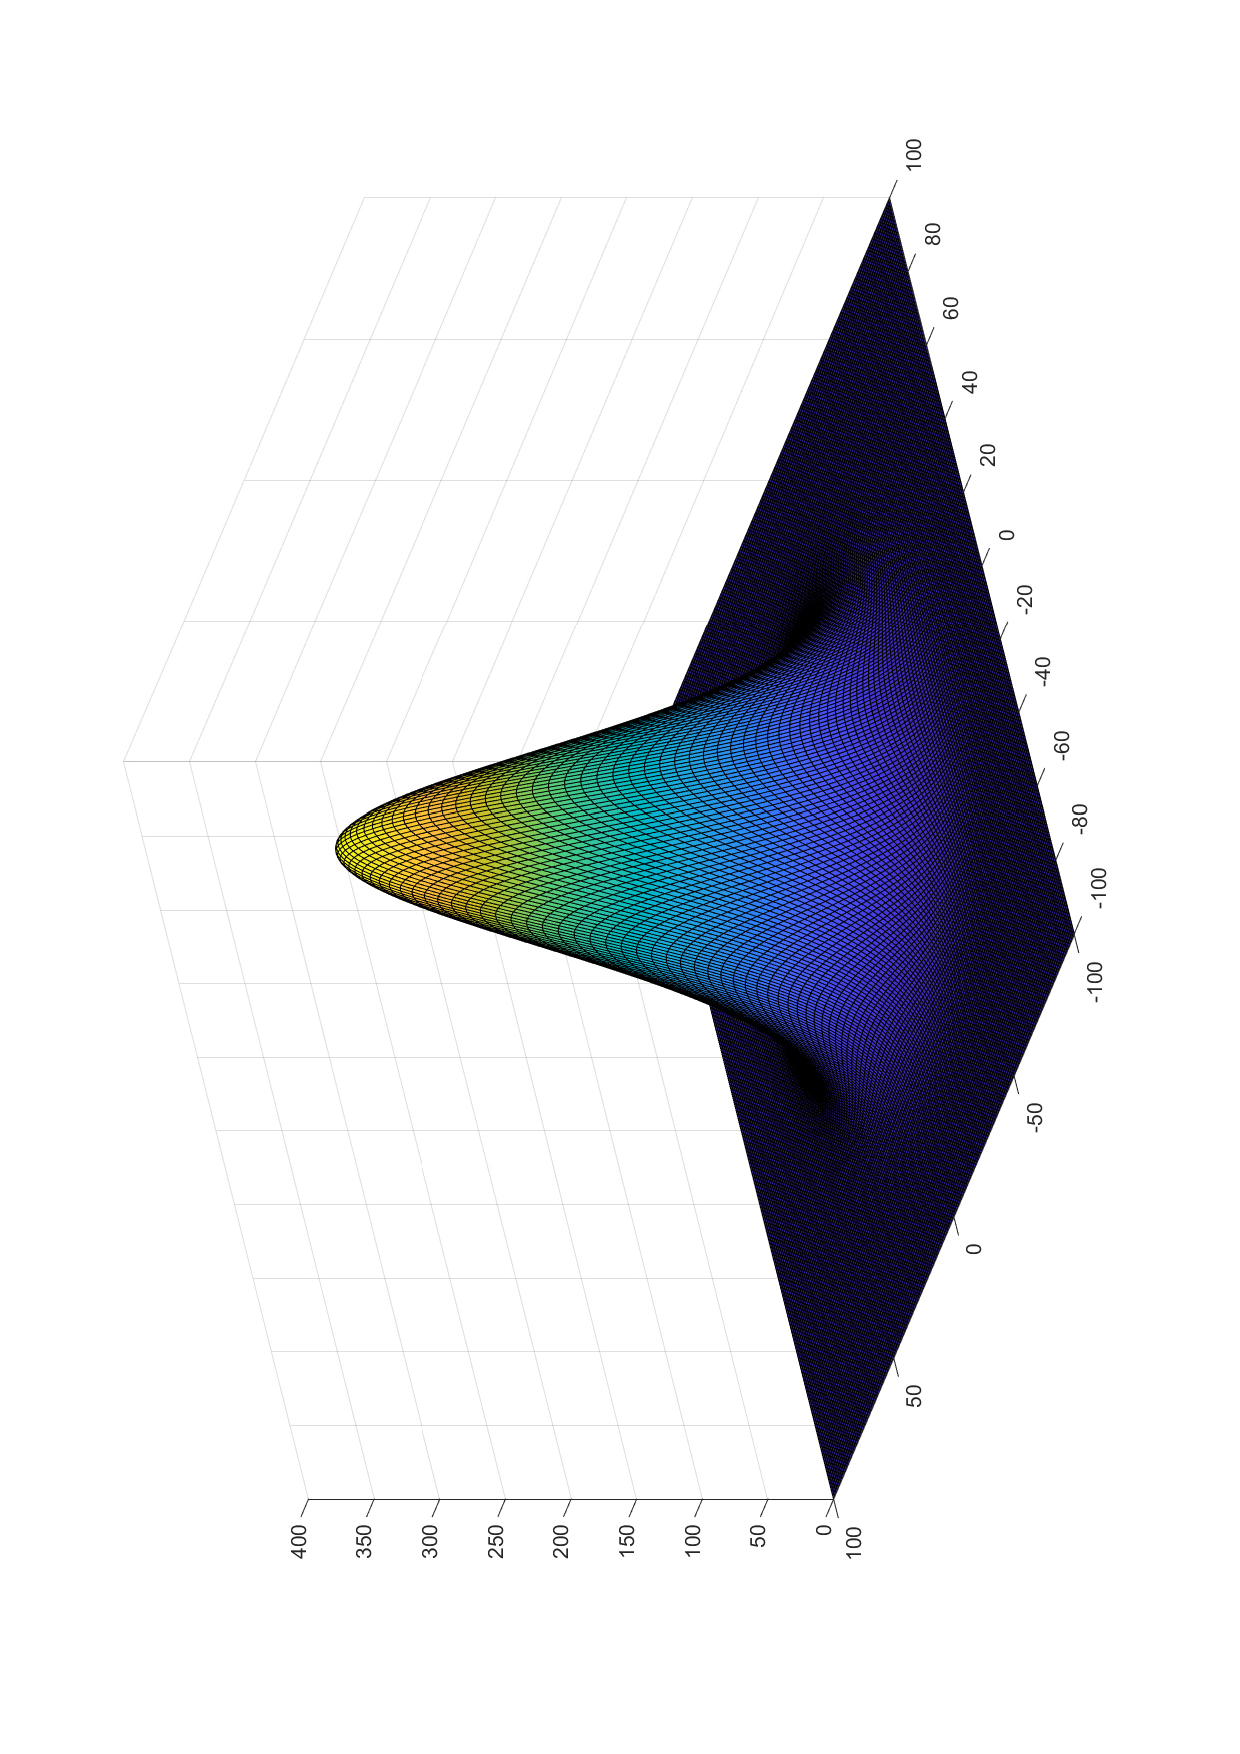
\includegraphics[width=0.8\textwidth,angle=-90]{grafiken/GaussKurve.pdf}
	\caption{Potentialfeld der gau�schen radialen Basisfunktion}
	\label{fig:PotRobotino}
\end{figure}

\subsection{Ziel} \label{sec:Ziel}
Das Ziel im Potentialfeld wird als Kegel mit konstantem Faktor realisiert. Dazu wird die in Gleichung \eqref{fun:H_Ziel} dargestellte Funktion genutzt. Um durch Tr�gheit verursachte Schwingungen um den Zielpunkt zu vermeiden, wird ein abstandsabh�ngiger Faktor als Filterung nachgeschaltet. Das Zielpotentialfeld ist in Abbildung \ref{fig:PotZiel} dargestellt.

\begin{align}
\label{fun:H_Ziel}
H_{Ziel}(x,y)= K \cdot \sqrt{(x-x_{Ziel})^2+(y-y_{Ziel})^2} 
 \end{align}
 
\begin{figure}
	\centering	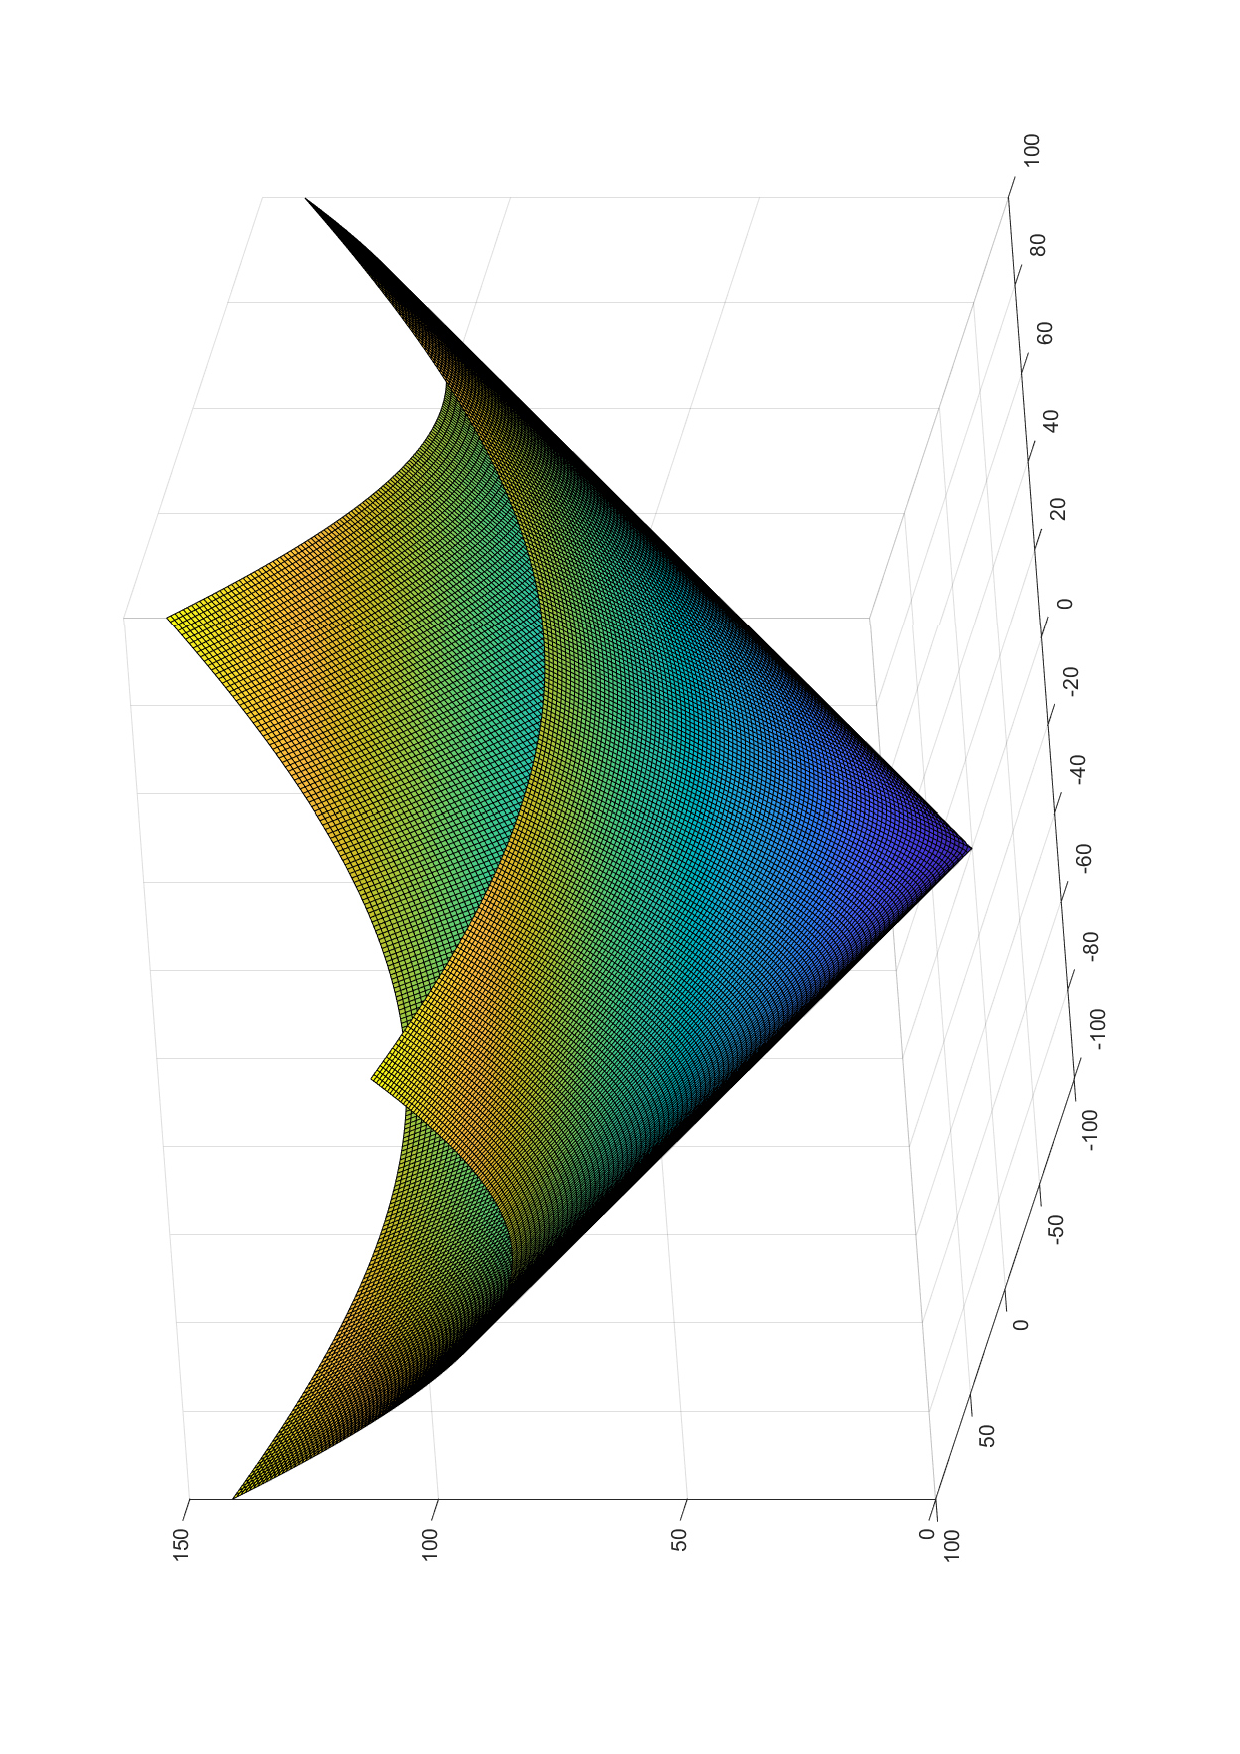
\includegraphics[width=0.8\textwidth,angle=-90]{grafiken/ZielKurve.pdf}
	\caption{Potentialfeld Ziel}
	\label{fig:PotZiel}
\end{figure}
\section{Kollisionsvermeidung durch kritische Bereiche}
Bei der Analyse des verwendeten Verfahrens zur Bahnplanung entstehen mehrere Bereiche, bei den die Potentialfeldmethode an ihre Grenzen st��t. Es treten lokale Minima auf, die nicht gleich mit dem Zielpunkt sind. Zwei Roboter k�nnen sich, bei gleichem Ziel, jeweils gegenseitig am Erreichen hindern. Hinter den Stationen und links von der ersten Station ist nicht gen�gend Platz zur perfekten Bahnplanung mittels Potentialen. W�rde ein anderer Robotino in die gleich Region fahren, ist die geplante Strecke nur noch schwer zu realisieren. Die Wahrscheinlichkeit, dass der Robotino gegen die Wand oder Station "gedr�ckt" wird steigt stark. \\
\\
Aus diesem Grund wurden hinter den Stationen Einbahnstra�en entworfen, in denen der Robotino gesch�tzt wieder in den freien Bereich gef�hrt wird. Hiermit wird jedoch noch nicht das Problem der Roboterbegegnung vor den Zielen verhindert.
\subsection{Selbstorganisation durch Wartebereiche}
\label{subsec:Selbstorga}
Um die Entstehung von lokalen Minima zu verhindern, wurde die Software der Robotinos um eine Selbstorganisation erweitert. 
Diese Erweiterung beinhaltet Wartepositionen, damit ein Roboter, der zur einer bereits besetzten Station fahren soll, sich au�erhalb des Kollisionsbereichs anstellt.
\begin{figure}[h]
	\centering
	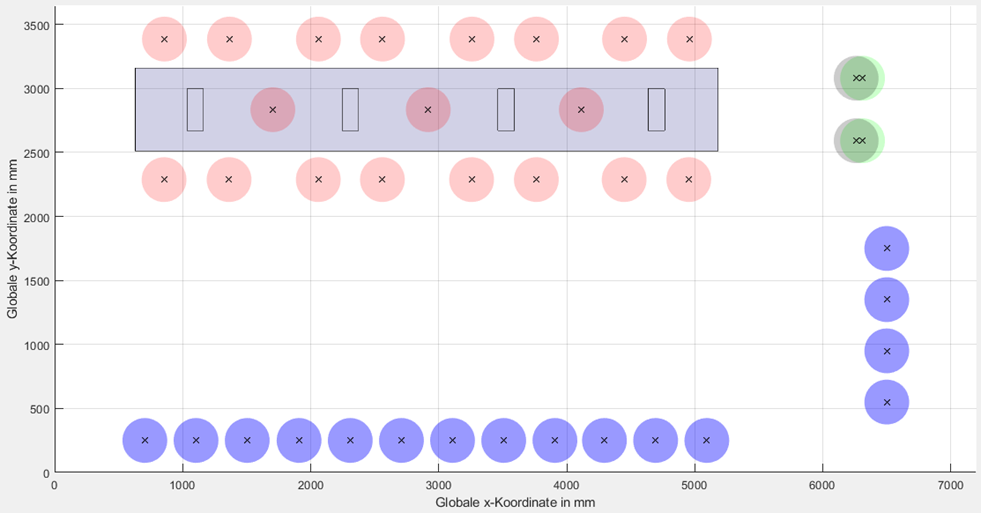
\includegraphics[width=0.5\textwidth]{Bilder/Lageplan.png}
	\caption{Lageplan der FIFO Pl�tze}
	\label{FIFOPlan}
\end{figure}
\\
In Abbildung \ref{FIFOPlan} erkennt man am unteren Rand der Karte zw�lf blaue Kreise, welche die Wartebereiche darstellen. Zu jeder Station geh�ren drei Wartepositionen. Durch sich ver�ndernde Z�hlweisen, ist der zugeh�rige Warteplatz zu einer Station immer eindeutig zuzuweisen. Im Kapitel \ref{cha:Implementierung} wird dies weiter erl�utert.\\
\\
\\
Mit Hilfe des UDP-Datenpaketes der Kameradaten ist es f�r einen Robotino m�glich die Positionen der anderen Robotinos zu erhalten. Ist nun die Zielstation bereits von einem anderen Robotino belegt, wird mit Hilfe der Selbstorganisationssoftware die erste m�gliche Wartepostion als Ziel �bernommen. Ist diese auch bereits belegt wird die Warteposition um einen Platz erh�ht.\\
Dem gesamten Anstellprozess liegt das \glqq First In First Out-Prinzip\grqq{} (im weiteren nur noch FIFO genannt) zu Grunde.
Dies bedeutet: Wer sich als erstes anstellt, darf auch als erstes wieder herausfahren.\\
Damit auch die Warteschlange beim Herausfahren eingehalten wird, wurde die Software ein weiteres mal erweitert.
Die Position der anderen Roboter wird in einem Merker gespeichert und erst zur�ckgesetzt, wenn der Roboter an der n�chsten Warteposition, beziehungsweise an der Zielposition, angekommen ist. Besonders das Freischalten der ersten Wartepostion ist kritisch. Wenn ein anderer Robotino die Zielstation verlassen hat, f�r diese Station aber mehr als ein Robotino wartet, w�rde beide Robotinos direkt zur Station fahren. Mit Hilfe des Merkers wird die erste Warteposition erst freigeschaltet, wenn der Robotino, der vorher in der ersten Wartepostion war, an der Zielstation angekommen ist. Das bedeutet, dass auch w�hrend der l�ngeren Strecke zwischen Wartepositionen und Stationen gesichert ist, dass nur ein Robotino gleichzeitig die Station anf�hrt. Ist der Roboter dort angekommen, wird die erste Wartepostion freigeschaltet und der Robotino auf dem zweiten Platz darf auf den ersten Platz vorfahren.\\
\\
Diese Warteschlange wird noch ein weiteres mal im Programmablauf abgefragt. Hat der Robotino seinen Auftrag abgearbeitet, also sein Werkst�ck abgeholt beziehungsweise abgelegt, wird die Belegung der Warteschlange zur zugeh�rigen Station abgefragt. Wartet dort bereits der n�chste Roboter f�hrt der Robotino nach Hinten, also zur Wand hin, aus der Station heraus. Von dort gelangt er �ber die Einbahnstra�en wieder in das freie Feld.\\
\\
Bei der Erweiterung des Projektes um einen f�nften Roboter, wie in Kapitel \ref{cha:Robo2.0} erkl�rt, wird die vierte Anstellposition nicht neben den anderen Wartepostionen generiert, sondern auf Grund von Platzmangel die Standbyposition einprogrammiert.
 
\subsection{Bekannte Hindernisse}
\label{subsec:bekannt}
Um generelle Begegnungen anderen Robotinos in der normalen Fahrzone zu vermeiden, wurde ein Ausweichman�ver entworfen. 
Befindet sich ein anderer Roboter im Bereich zwischen den gesteuerten Roboter und seinem Ziel und in einer Entfernung von 20 cm wird auf den Zielvektor eine $90^\circ$-Drehung addiert. Der Robotino f�hrt somit f�r eine kurze Zeit mit gleichbleibendem Abstand zum Ziel. Ist der behindernde Robotino nicht mehr im gef�hrdeten Bereich, wird wieder der normale Zielvektor eingestellt.\\
\\
F�r eine hohe Dynamik im Gesamtsystem unterscheidet die Software zwischen sich bewegenden und stehenden Robtinos. Anhand der Kameradaten werden die aktuellen Positionen mit deren vorherigen mittels Merker verglichen. Ist die Differenz gr��er der definierten Toleranz, bewegt sich der Robotino. Sich bewegende Robotinos stelle eine gr��ere Kollisionsgefahr dar. Deshalb werden die Potentialfelder jener Robotinos vergr��ert. Der gesteuerte Roboter wird somit in einem gr��eren Abstand vorbei fahren.

\subsection{Unbekannte Hindernisse}

Das verbaute Kamerasystem ist nicht in der Lage andere Objekte, au�er die mit Aruko-Markern versehenden Robotinos, zu erkennen. Um jedoch auch eine Kollision mit Menschen zu verhindern besitzt der Robotino neun Infrarot-Sensoren gleichm��ig um den untersten Rand des Roboters verteilt. Detektiert einer der Sensoren ein Objekt ermittelt die Software an welcher Stelle das Objekt erkannt wurde und manipuliert den Zielvektor. Es wird ein um $180^\circ$ gedrehter Zielvektor ein programmiert.
Hat sich das unbekannte Hindernis entfernt, wird wieder der normale Zielvektor geschaltet.
\newpage
\section{Schnittstellen}
Im gesamten Projektablauf ist die Kommunikation mit anderen Gruppen ausschlaggebend f�r eine perfektes Gesamtkonzept.
In der Bahnplanung wurde vor allem mit der Gruppe der Bahnregelung und mit der Gruppe der Fertigungsplanung eng zusammengearbeitet.
\subsection{Bahnregelung}\label{sec:Kon_Bahnregelung}
In sehr engen Bereichen, in denen auch eine hohe Pr�zision erforderlich ist, st��t die Potentialfeldmethode an ihre Grenzen. Aus diesem Grund wurde der gesamte Bereich direkt am Anfang des Projektes aufgeteilt. Das Potentialfeld wird in den freien Bereiche benutzt und an den Randbereichen des Feldes. Das Anfahren der einzelnen F�cher innerhalb der Stationen, sowie das Werkst�ckhandling, ist an die Bahnregelung �bergeben worden.\\
\\
In Abbildung \ref{FIFOPlan} stellen die acht roten Kreise vor den Stationen die �bergabepunkte dar. Befindet sich der Robotino innerhalb eines solchen Kreises, inklusive einer gewissen Toleranz, wird ein �bergabebit gesetzt und die Bahnregelung �bernimmt das pr�zise Anfahren zuerst des RFID Leseger�tes und anschlie�end das Ablegen in ein Stationsfach. ( Beim Abholen ist der Prozess andersherum.)
Somit geh�ren zur Schnittstelle nicht nur das �bergabebit. Die Gruppe der Bahnregelung ben�tigt dar�ber hinaus auch noch den genauen Auftrag der Fertigungsplanung. Hat die Bahnregelung den Auftrag abgearbeitet, wird der �bergabebit am �bergabepunkt getoggelt und der Robotino f�hrt wieder im Potentialfeld. Dieser �bergabepunkt ist variabel, wie bereits in dem Unterkapitel \ref{subsec:Selbstorga} erl�utert.\\
\\  
Da die Bahnregelung sehr pr�zise die Position des Robotinos f�r eine hoch genaue Fahrt ben�tigt, wurde von der Gruppe ein Kalman-Filter f�r die Robotino Position entworfen. Ohne Beobachter sendet die Kamera, bei nicht Erkennung eines Robotinos, die Positionsdaten [0,0] f�r diesen Robotino. Diese falsche Postion kann zu einigen Fehlern in den Berechnungen f�hren. Dieser Beobachter erm�glicht eine Fehlerfreie Positionsdarstellung des Roboters auch bei kurzzeitiger Verdeckung des ArUcomarkers. Die Beobachterdaten werden auch in der Bahnplanung durchgehende verwendet. 
\newpage
\subsection{Fertigungsplanung}\label{sec:Kon_Fertigungsplanung}
Die Fertigungsplanung ist f�r die gesamte Simulation der Fabrikumgebung zust�ndig. In der Gruppe werden verschiedene Auftr�ge generiert und intelligent auf die vier Robotinos verteilt. Mittels UDP-Kommunikation wird der jeweilige Auftrag an den jeweiligen Roboter gesendet.
\begin{figure}[h]
	\centering
	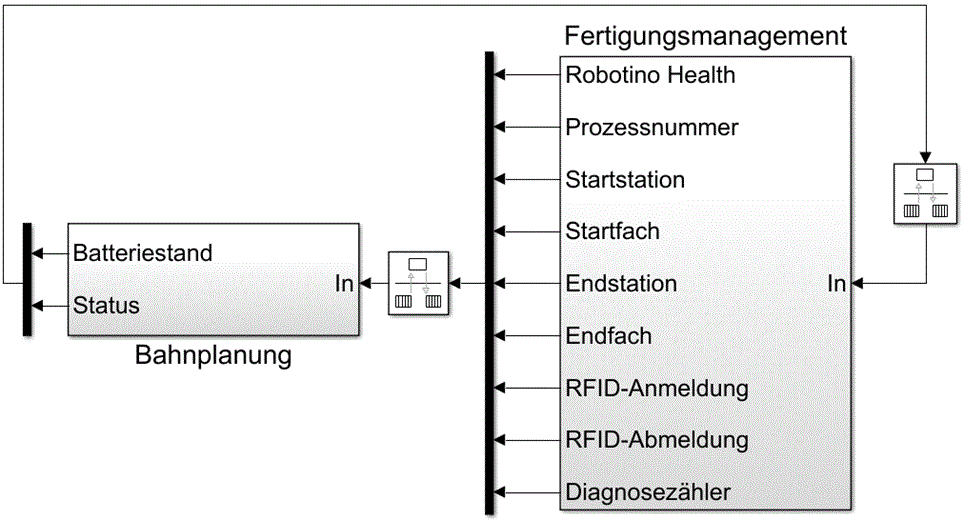
\includegraphics[width=0.6\textwidth]{Bilder/Schnittstelle_Fertigungsplanung.png}
	\caption{Schnittstelle mit der Fertigungsplanung}
	\label{pic:SchnittstelleGewerk1}
\end{figure}
\noindent
In Abbildung \ref{pic:SchnittstelleGewerk1} ist der Informationsaustausch dargestellt. Die Informationen, die die  Bahnplanung an die Fertigungsplanung zur�cksendet, wurden um einen weiteren Punkt erweitert. Die Ist-Position des Roboters wird ebenfalls gesendet. Diese Position wird von der Fertigungsplanung f�r die Fabriksimulation ben�tigt. Im Statusbyte wird �bermittelt, was der Robotino zu dem Zeitpunkt gerade ausf�hrt. Also ob er im Potentialfeld f�hrt oder eine Station anf�hrt, etwas ablegt oder etwas aufnimmt. Dar�ber hinaus werden im Status auch Fehlermeldungen weitergeleitet, dazu im Unterkapitel \ref{Fehlererkennung} mehr.\\
\\
Von der Fertigungsplanung bekommt das Programm den genauen Auftrag, den der Robotino abarbeiten soll. Jeder neue Auftrag erh�lt auch eine neue Prozessnummer. Der Auftrag besteht aus der Startstation mit zugeh�rigem Fach, an dem ein Werkst�ck abgeholt werden und in welches Fach von welcher Station es gebracht werden soll. 
Damit jedes individuelle Werkst�ck auch entsprechend erkannt wird, sind an jeder Station RFID Lese-/Schreibk�pfe angebracht. Wird ein Werkst�ck in die jeweilige Station gebracht, wird es dort angemeldet. Beim  Aufnehmen wird es abgemeldet. Hierf�r werden zwei Bytes in der Schnittstelle verwendet. Die Information �ber die einzelnen Werkst�cke werden von der Fertigungsplanung verarbeitet und in einer Cloud gespeichert.\\
\newpage

\subsection{Fehlererkennung}
\label{Fehlererkennung}

Eine weitere �bergabeinformation zwischen den drei Gruppen ist das Fehlerhandling. Es wird zwischen drei verschiedenen Fehlern des Robotinos unterschieden:
\begin{enumerate}
\label{Fehlerliste}
\item Kein Werkst�ck vorhanden
\item Stationsfach belegt
\item Werkst�ck verloren
\end{enumerate}
\noindent
Beim Anfahren eines Stationsfachs zur Aufnahme eines Werkst�ckes durch die Bahnregelung, wird zwischen den Greifern eine Lichtschranke abgefragt. Kann kein Werkst�ck aufgenommen werden, weil beispielsweise kein Werkst�ck erkannt wurde, wird ein Fehler ausgel�st. Dieser Fehler wird anschlie�end an die Fertigungsplanung gesendet. Die Fertigungsplanung entscheidet dann, ob ein falscher Auftrag gesendet wurde oder in der 'Fabrik' ein Fehler vorliegt, welcher per manuellen Eingriff behoben werden muss. 
Der zweite Fehler wird �ber einen Z�hler der Anfahrversuche f�r ein Fach realisiert. Schafft es der Robotino innerhalb von drei Anfahrversuchen nicht das Werkst�ck abzulegen, so wird der zweite Fehler gesendet. 
Verliert der Roboter w�hrend der Fahrt das Werkst�ck, wird der dritte Fehler gesendet. Hier muss manuell das Werkst�ck aus dem Fahrbereich entfernt werden.
%\subsection{Roboter Umwelt}
%\subsection{Robotino}
%\subsection{Ziel}
%\section{Kollisionsvermeidung durch *ich kann nicht lesen was davor steht* Bereiche}
%\subsection{Selbstorganisation durch Wartebereiche}
%\subsection{Bekannte Hindernisse}
%\subsection{Unbekannte Hindernisse}
%\section{Schnittstellen}
%\subsection{Bahnregelung}
%\subsection{Fertigungsplanung}
%\subsection{Positionsdaten}
%\section{Gesamtprogrammablauf}
%\chapter{Simulation und Testplanung}
\chapter{Simulation und Testplanung}
Um das Potentialfeld auch ohne Robotinos zu testen, wird zu Beginn des Projektes mit einer vereinfachten Simulation das Potentialfeld auf Ihre Funktionsf�higkeit gepr�ft. Bei dieser Simulation wird der Robotino als enfache I-Strecke betrachtet. Dabei wird der Ausgang der Strecke auf den Istpositionsinput gegeben und der berechnete Geschwindigkeitsvektor auf die Strecke gegeben. Desweiteren werden auf die restlichen Inputs Konstanten gegeben und die Ausgangsdaten in einer Logdatei abgespeichert. Da nach wenigen Versuchen erkennbar ist, dass das Potentialfeld seine Funktion erf�llt, wird im folgenden mit dem Robotinos direkt getestet. Dazu wird zu Beginn der Fertigungsbereich nicht betrachtet und nur ein Festprogrammiertes Ziel angefahren. Um flexibel Ziele anfahren zu k�nnen und die Schnittstelle mit der Fertigungsplanung zu teseten wird ein UDP-Dummy in Simulink erstellt mit dem Auftr�ge an den Robotino per UDP in Simulink gesendet werden k�nnen. Dadurch k�nnen mehrere Ziele hintereinander Angefahren werden. Im n�chsten Schritt wird die Schnittstelle mit der Bahnregelung gestestet dazu werden beide Simulinkmodelle kombiniert und auf den Robotino geladen. Dadurch k�nnen Schnittstellenprobleme zwischen der Bahnregeleung und der Bahnplanung fr�hzeitig behoben werden. Da sich im laufe des Projektes gezeigt hat, dass die Fertigungsplanung den Gesamtsystemtesttermin nicht einhalten kann, wird der UDP-Dummy in zusammenarbeit mit der Bahnregelung dahingehend erweitert, zufallsgenerierte Auftr�ge zu senden. Im letzten Schritt wird der UDP-Dummy als Fertigungsplanungsersatz erweitert indem sich die Positionen der Werkst�cke gemerkt wird und die zufallsgenerierten Auftr�ge auf ausf�hrbare Auftr�ge gefiltert wird. Zum Ende des Projektes wird zus�tzlich eine Simulation, wie zu Beginn, mit der Erweiterung auf 5 Robotinos ausgef�hrt um geringe �nderungen im Programm aufzuzeichnen, da die Aufzeichnung von Daten von mehreren Robotinos unter Simulinkrealtime einige Probleme verursacht. Unter Kapitel \ref{} wird eine Simulation des Ausweichman�vers dargestellt.
\section{Simulation des Ausweichman�vers}
In diesem Abschnitt wird die Simulation des Ausweichman�vers dargestellt. Dazu werden zwei Simulationen miteinander Verglichen. In der ersten Simulation, welche in Abbildung \ref{fig:SimulationAusweich} dargestellt ist, werden zwei Robotinos betrachtet. Robotino 1 in Rot dargestellt f�hrt von der Position [500 1000] zur Station 7 welche sich ganz rechts befindet. Robotino 2 in blau dargestellt f�hrt von der Position [4500 1000] zur Station 0 welche sich ganz links befindet. Wie in der Abbildung zu sehen ist, umfahren sich die Robotinos rechts herum.

\begin{figure}
	\centering	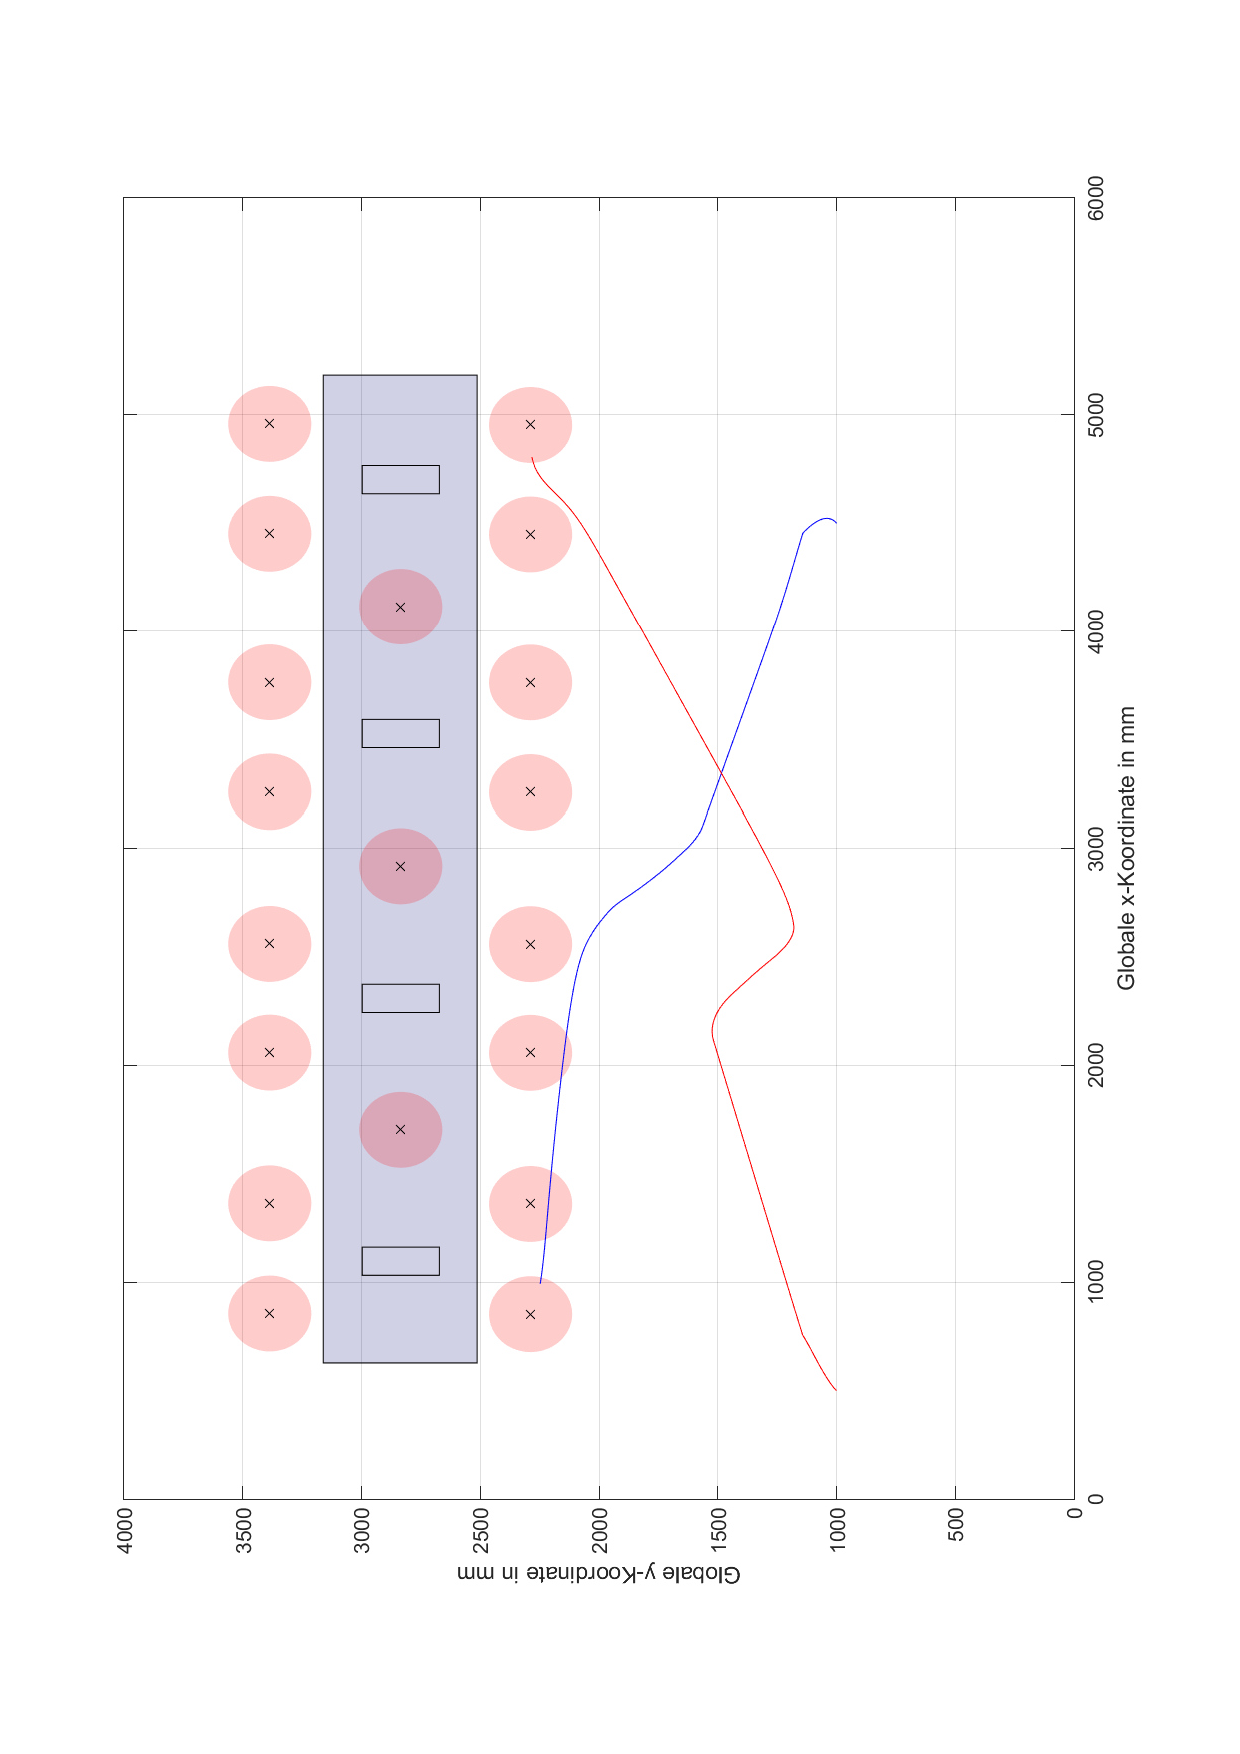
\includegraphics[width=0.5\textwidth,angle=-90]{grafiken/SimulationAusweich.pdf}
	\caption{Simulation mit Ausweichfunktion}
	\label{fig:SimulationAusweich}
\end{figure}

 In der zweiten Simulation, welche in Abbildung \ref{fig:SimulationohneAusweich} dargestellt ist, werden die gleichen Robotinos mit der gleichen Start und Zielposition betrachtet. In dieser Simulation wird jedeglich die Ausweichfunktion auf Null gesetzt. Wie in der Abbildung zu erkennen ist, kommt es zu einem Absto�verhalten, wodurch die Robotinos stark ausgebremst werden. Wie in den Abbildungen zu erkennen ist, hat die entwickelte Ausweichfunktion eine Verbesserung im Ausweichverhalten verursacht.
 
\begin{figure}
	\centering	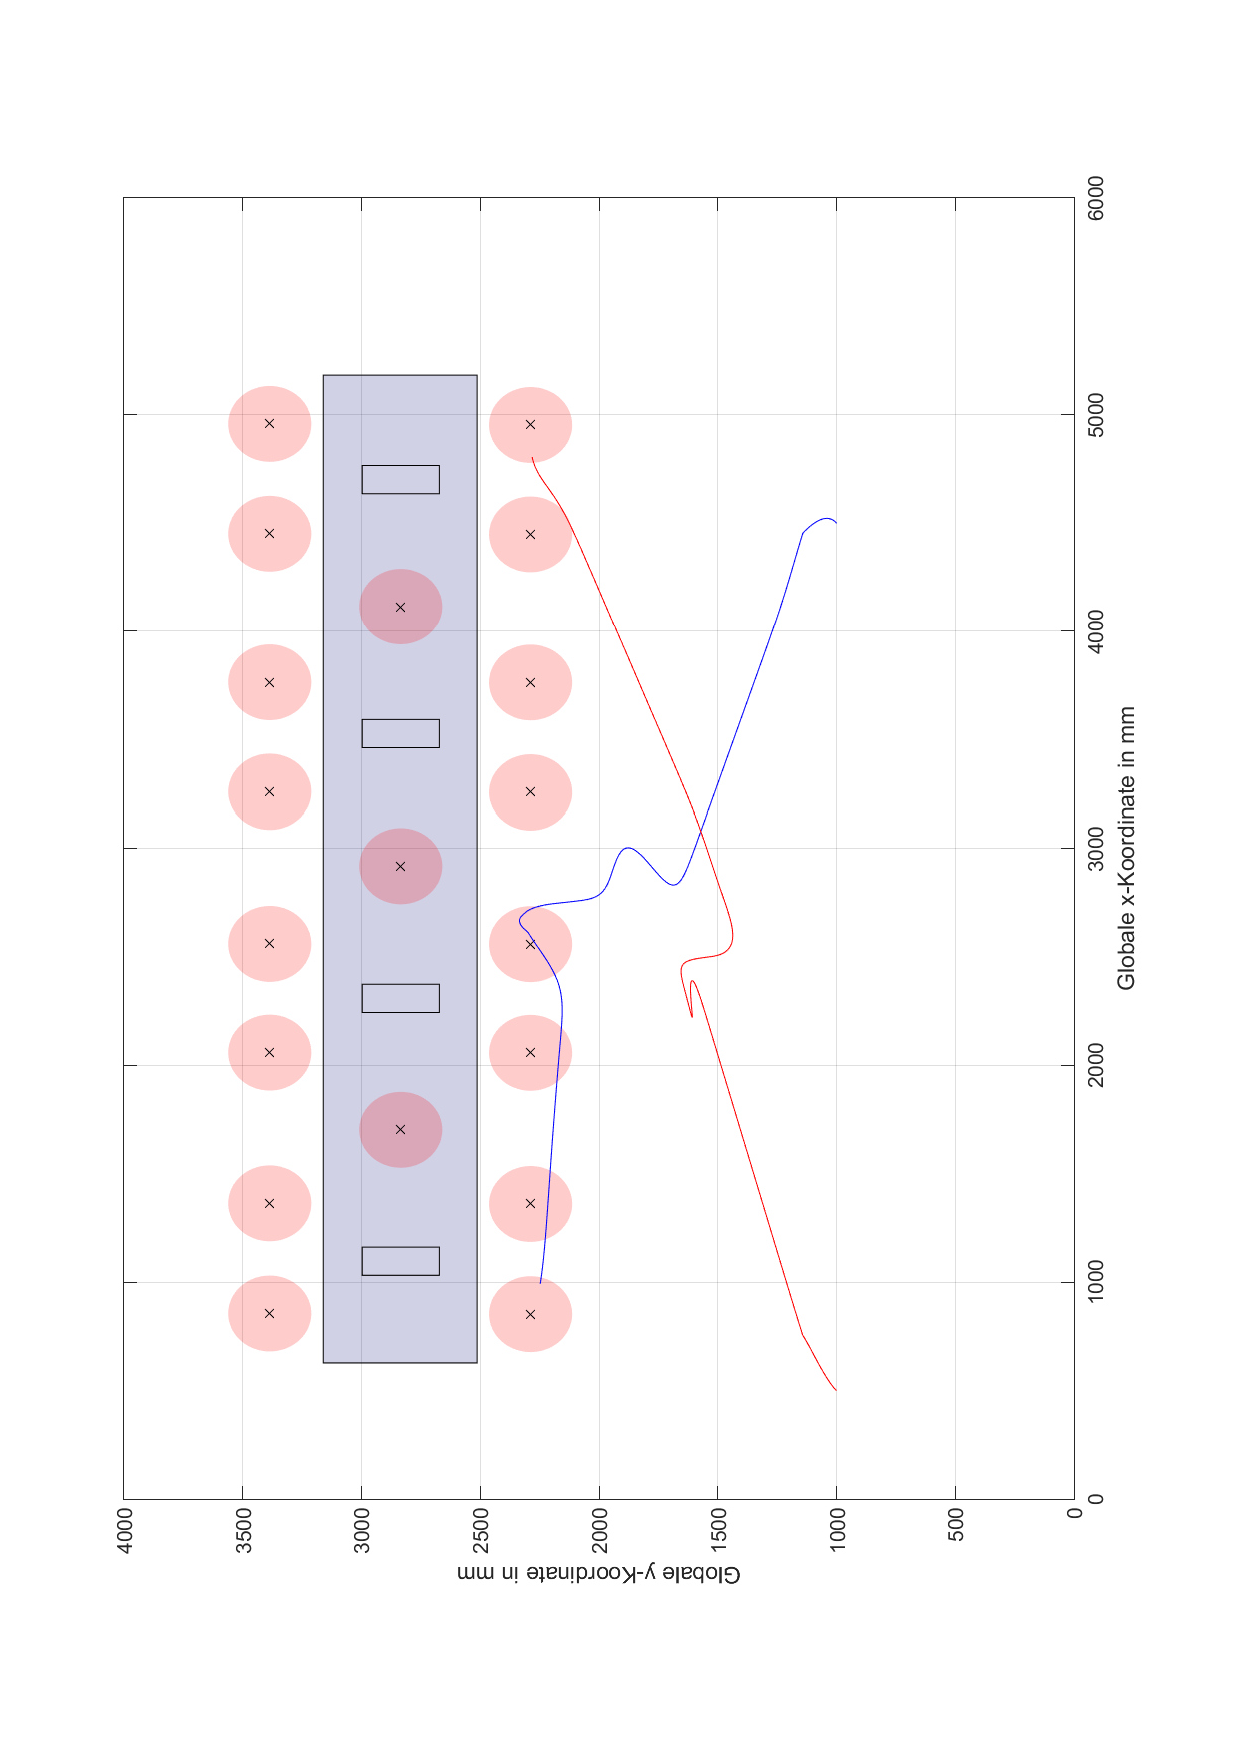
\includegraphics[width=0.5\textwidth,angle=-90]{grafiken/Simulation_ohne_Ausweich}
	\caption{Simulation ohne Ausweichfunktion}
	\label{fig:SimulationohneAusweich}
\end{figure}
\section{Simulation Wartebereiche}
%\chapter{Implementierung und Zielsysteme}
\chapter{Implementierung und Zielsysteme}
\label{cha:Implementierung}
In diesem Kapitel wird die Umsetzung der einzelnen Algorithmen des in Kapitel \ref{cha:konzept} erl�uterten Konzepts mit Hilfe der Software Matlab/Simulink erkl�rt.
F�r einen besseren �berblick zu dem Konzept zeigt die Abbildung \ref{Ablaufdiagramm} ein Ablaufdiagramm des Programms der Bahnplanung.\\

\begin{figure}[h]
	\centering
	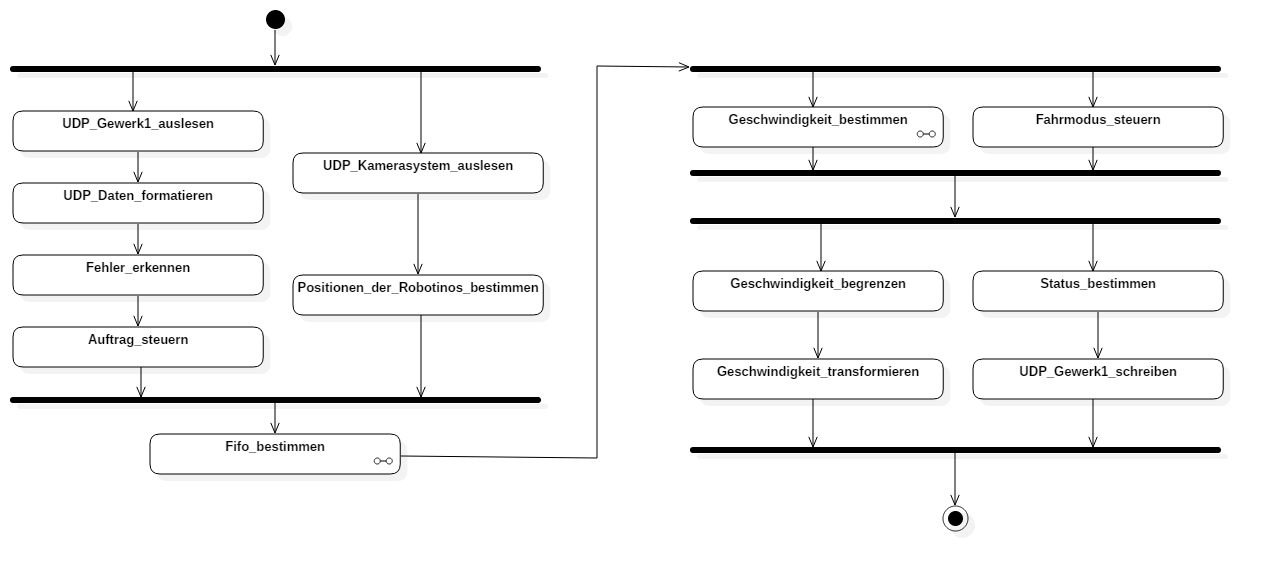
\includegraphics[width=0.9\textwidth]{Bilder/Bahnplanung.png}
	\caption{Ablaufdiagramm Konzept}
	\label{Ablaufdiagramm}
\end{figure}
\noindent
Zun�chst wird der Auftrag der Fertigungsplanung verarbeitet und parallel dazu wird die eigene Position des Robotinos sowie die Positionsdaten der anderen Robotinos bezogen. Nachdem die Selbstorganisation durch Wartebereiche abgearbeitet wurde, wird das erhaltene Ziel weitergeleitet. Mit dem bekannten Ziel wird der Zielvektor bestimmt. Die Hinderniserkennung l�uft nun gleichzeitig.
Hat der Robotino sein Endziel erreicht, kann ein neuer Auftrag abgearbeitet werden.\\
\\Hat ein Robotino zur Zeit keinen Auftrag, wird als Ziel die Standby-Position einprogrammiert. Zun�chst wird der Grundalgorithmus zur Zielgebung erl�utert und anschlie�end um die einzelnen Unterpunkte des Konzeptes erweitert.\\


\section{Selbstorganisation durch Wartebereiche}
\label{sec:Impl:Selbstorga}
Die in dem Unterkapitel \ref{subsec:Selbstorga} erkl�rte intelligente Selbstorganisation wird im Folgenden erkl�rt und es wird gezeigt, wie der Algorithmus in der Software Simulink umgesetzt wird. \\
\\
Das Ablaufdiagramm in Abbildung \ref{AblaufdiagrammFIFO} stellt den Ablauf des Algorithmus dar.\\

\begin{figure}[h]
	\centering
	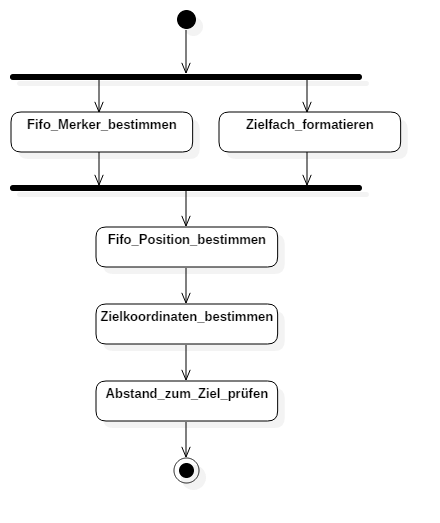
\includegraphics[width=0.4\textwidth]{Bilder/FIFO_Steuerung.png}
	\caption{Ablaufdiagramm der Selbstorganisation}
	\label{AblaufdiagrammFIFO}
\end{figure}
\noindent
\\
Die Positionen der anderen Robotinos werden �ber den 'FIFO Merker' gepr�ft und es wird geschaut, ob die anderen Roboter Positionen einnehmen, die ein zugeh�riger Warteplatz f�r die Zielstation darstellen.\\
Die Roboterpositionen werden in einem Array der X- Positionen und einem der Y-Postionen gespeichert. Die 12 bestehenden in gleichm��igen Abstand aufgeteilten Wartebereiche k�nnen mit der Formel \ref{equ:wartebereiche} in Zeile 8 des Matlab-Codes \ref{Fifomerker} in X-Richtung berechnet werden.\\
\begin{align}
\label{equ:wartebereiche}
  N(n)=round((X(n)-703)/400)+1;
  \end{align}  
Stimmen die X-Positionen der Robotinos mit den Bereichen �berein und sind die Y-Positionen am linken Rand des gesamten 'Fabrik'-Bereiches, wird der Wartebereich an dem sich ein Robotino befindet, mit einer jedem Robotino spezifischen Nummer belegt.
Damit die Wartebereiche auch in jedem Zyklus wieder neu berechnet werden, wird der Merker zun�chst auf null gesetzt und in jedem Zyklus mit neuen Werten beschrieben.\\

\begin{lstlisting}[caption={FIFO Merker},label=Fifomerker,basicstyle=\small]
function [FifoArray1,StationArray1,LadeArray1]= fcn(Robbi,FifoArray,LadeArray)
X=[Robbi(1) Robbi(4) Robbi(7) Robbi(10)];
Y=[Robbi(2) Robbi(5) Robbi(8) Robbi(11)];
FifoArray1=zeros([1 12]);
FifoArray1=FifoArray(1:12);
N=zeros([1 5]);
for n= 1 : 1 : 4
        N(n)=round((X(n)-703)/400)+1; % Berechnung in welchem Fifo der Roboter sich befinde
elseif (Y(n)<450 && (X(n)>100 && X(n)<5250)&& N(n)<=12 && N(n)>0)
        for i=1:12
            if FifoArray1(i)==n
                FifoArray1(i)=0;
            end
        end
            FifoArray1(N(n))=n;
          ...
          ...
end
\end{lstlisting}
Auch die Belegung der Stationen wird mit dem selben Algorithmus berechnet. Einzig die Bereichsabfrage �ndert sich und die Formel \ref{equ:wartebereiche} f�r die Berechnung der Belegung. Hierbei �ndert sich allerdings nur die Unterteilung und der Offset der Formel.\\
Die Merkerwerte werden in einem Stateflowdiagramm weiterverarbeitet. Die Eing�nge des Stateflowdiagramms sind die Auftragsdaten, die Merkerdaten, und die genauen Positionsdaten des Robotinos aus Beobachter und Kamerawerten.
Damit das System die Wartepositionen der zugeh�rigen Zielstationen f�r die Zuweisung verwendet, wird die Formel \ref{equ:ersterfifo} benutzt. Die zw�lf Wartebereiche k�nnen so explizit den acht Stationen zugeordnet werden. Zwei Stationen teilen sich jeweils drei Wartebereiche.
\begin{align}
\label{equ:ersterfifo}
 &ersterFifo=floor(Zielstation/2)\cdot3+2 \cdot mod(Zielstation,2)+1\\
 &zweiterFifo=floor(Zielstation/2)\cdot 3+1+1\\
 &dritterFifo=floor(Zielstation/2)\cdot 3+2-2\cdot mod(Zielstation,2)+1
  \end{align} 
Ist der erste Bereich belegt wird der zweite Bereich abgefragt ist dieser belegt wird der Dritte abgefragt. Sind alle drei Bereich belegt, gibt das Stateflowdiagramm den h�chsten Wert aus. Beim h�chsten Wert wird die Standbyposition als Ziel einprogrammiert.\\
\\

Wird im n�chsten Zyklus der n�chst kleinere Wartebereich frei, so wird dieses als Ziel angefahren. 
In dem Fall, wenn ein anderer Robotino den ersten Wartebereich verl�sst und zur Zielstation f�hrt, besteht ein Sonderfall. Da die Strecke zwischen den beiden Punkten ca. zwei Meter betr�gt dauert diese Fahrt mehrere Zyklen. Damit ein dahinter stehender Robotino in dem Moment nicht auch direkt die Station anf�hrt, weil alle anderen Bereiche frei sind, wird eine weitere Position abgefragt. Die Stationsbelegung wird abgefragt. 
Die Station wird erst wieder freigegeben, wenn sie im Stationsmerker nicht mehr belegt ist.\\

\section{Bekannte Hindernisse}
\label{sec:bekHindernis}

F�r eine verbesserte Kollisionsvermeidung wurde das Ausweichman�ver, wie in Unterkapitel \ref{subsec:bekannt} bereits erkl�rt, verwendet. Die Aufgabe des Man�vers ist es den Zielvektor des Robotinos so zu ver�ndern, dass er einem sich im Weg befindenden Robotino mit einem gr��eren Abstand ausweicht.
Es werden die Position des Robotinos ben�tigt sowie die Positionen der anderen Robotinos, die St�rpositionen. Dar�ber hinaus ben�tigt das Man�ver den Zielvektor.\\
Zun�chst wird analysiert in welchem Winkel die St�rpositionen sich zum Zielvektor befinden. Liegt ein anderer Robotino innerhalb von \ang{30} zum Zeilvektor wird ein Ausweichwinkel berechnet. 
\begin{align}
\label{Ausweichwinkel}
Ausweich(1,i)=+asin(Abstand(2,i)/Hyp)-pi/2
\end{align}
Der erste Wert des Ausweichs-Array aus Formel \ref{Ausweichwinkel} ist der Ausweichwinkel. �ber eine trigonometrische Funktion wird der genaue Winkel des Zielvektors zum Ziel ausgerechnet und \ang{90} addiert.
Solange eine St�rposition innerhalb der \ang{30} liegen, bleibt der Ausweichwinkel erhalten. Ist der im Weg liegende Roboter weit genug umfahren, wird der originale Zielvektor einprogrammiert.

\section{Unbekannte Hindernisse}
 \label{sec:unbekHindernis}
Unbekannte Hindernisse werden nur mit Hilfe der neun verbauten Infrarotsensoren erkannt. Zyklisch werden diese Sensoren abgefragt. Detektiert einer der Sensoren ein Hindernis wird zun�chst �berpr�ft, an welcher Position relativ zur Roboterausrichtung sich das Hindernis befindet. Der Ablauf wird im Code \ref{infra} dargestellt:\\
\begin{lstlisting}[caption=Infraroterkennung,label=infra,basicstyle=\small]
for x=1:9
 if  (isnan(IRDaten(x))==0) && (IRDaten(x) <= 150)
  IRWerte(1,x)=cos(((x-1)*40*pi/180)+RobPos(3))*(IRDaten(x)+200)+RobPos(1);
  IRWerte(2,x)=sin(((x-1)*40*pi/180)+RobPos(3))*(IRDaten(x)+200)+RobPos(2);
 else
  IRWerte(1,x)=NaN;
  IRWerte(2,x)=NaN;
 end
end
\end{lstlisting}
\noindent 
Wurde ein Hindernis detektiert, wird das Hindernis in globalen Koordinaten bestimmt. Diese berechneten 'IRWerte' werden anschlie�end in der Zielvektorberechnung aus Kapitel \ref{sec:potentialfeld} einbezogen.

\section{Potentialfeld}
\label{sec:potentialfeld}

Um das unter Kapitel \ref{sec:Potential} beschriebene Potentialfeldkonzept in Matlab/Simulink umzusetzten, werden die Funktionen \eqref{fun:H01} bis \eqref{fun:H5} partiell nach x und y abgeleitet. Die dabei entstehenden Funktionen sind als \eqref{fun:VxStation} bis \eqref{fun:VyZone5} definiert. Durch die Ableitung des Potentialfeldes ergibt sich der Gradient, der negiert werden muss, damit der ermittelte Vektor Richtung Ziel zeigt.

\scalebox{0.666}{\begin{minipage}{1.5\textwidth}
\begin{align}
\label{fun:VxStation}
Vx_{Hindernis}(x,y)=-K\cdot e^{-\frac{(x-Stationsposition_x)^2+(y-Stationsposition_y)^2}{2\cdot \sigma^2}} \cdot \frac{x-Stationsposition_x}{2\cdot \sigma^2}\\
\label{fun:VyStation}
Vy_{Hindernis}(x,y)=-K\cdot e^{-\frac{(x-Stationsposition_x)^2+(y-Stationsposition_y)^2}{2\cdot \sigma^2}} \cdot \frac{y-Stationsposition_y}{2\cdot \sigma^2}\\
\label{fun:VxZiel}
Vx_{Ziel}(x,y)=\frac{K\cdot(x-Ziel_x)}{\sqrt{(x-Ziel_x)^2+(y-Ziel_y)^2}}\\
\label{fun:VyZiel}
Vy_{Ziel}(x,y)=\frac{K\cdot(y-Ziel_y)}{\sqrt{(x-Ziel_x)^2+(y-Ziel_y)^2}}\\
\label{fun:VxZone01}
Vx_{Umwelt(Zone=0,x=0..5500,y=0..2500)}(x,y)=\frac{1}{\sigma}\cdot K \cdot e^{\frac{-x}{\sigma}} +\frac{-1}{\sigma}\cdot K \cdot e^{\frac{x-x_{max}}{\sigma}}\\
Vy_{Umwelt(Zone=0,x=0..5500,y=0..2500)}(x,y)=\frac{-1}{\sigma} \cdot K \cdot e^{\frac{y-2500}{\sigma}} +\frac{1}{\sigma} \cdot K \cdot e^{\frac{-y}{\sigma}}\\
Vx_{Umwelt(Zone=0,x=5500..x_{max},y=0..2500)}(x,y)=\frac{1}{\sigma}\cdot K \cdot e^{\frac{-(x-5500)+(y-2500)}{\sigma}} +\frac{-1}{\sigma}\cdot K \cdot e^{\frac{x-x_{max}}{\sigma}}\\
Vy_{Umwelt(Zone=0,x=5500..x_{max},y=0..2500)}(x,y)=\frac{-1}{\sigma} \cdot K \cdot e^{\frac{-(x-5500)+(y-2500)}{\sigma}} +\frac{1}{\sigma} \cdot K \cdot e^{\frac{-y}{\sigma}}\\
Vx_{Umwelt(Zone=0,x=5500..x_{max},y=2500..y_max)}(x,y)=\frac{1}{\sigma}\cdot K \cdot e^{-\frac{x-5500}{\sigma}} +\frac{-1}{\sigma}\cdot K \cdot e^{\frac{x-x_{max}}{\sigma}}\\
Vy_{Umwelt(Zone=0,x=5500..x_{max},y=2500..y_{max})}(x,y)=\frac{-1}{\sigma} \cdot K \cdot e^{\frac{y-y_{max}}{\sigma}} +\frac{1}{\sigma} \cdot K \cdot e^{\frac{-y}{\sigma}}\\
Vx_{Umwelt(Zone=1)}(x,y)=K_{gerade}\\
Vy_{Umwelt(Zone=1)}(x,y)=-2\cdot \frac{y-3500}{K_{parabel}}\\
Vx_{Umwelt(Zone=2)}(x,y)=-K_{gerade}\\
Vy_{Umwelt(Zone=2)}(x,y)=-2\cdot \frac{y-3500}{K_{parabel}}\\
Vx_{Umwelt(Zone=3)}(x,y)=-2\cdot \frac{x-300}{K_{parabel}}\\
Vy_{Umwelt(Zone=3)}(x,y)=-K_{gerade}\\
Vx_{Umwelt(Zone=4)}(x,y)=0\\
Vy_{Umwelt(Zone=4)}(x,y)=K_{gerade}\\
Vx_{Umwelt(Zone=5)}(x,y)=-2\cdot \frac{x-5500}{K_{parabel}}\\
\label{fun:VyZone5}
Vy_{Umwelt(Zone=5)}(x,y)=-K_{gerade}
 \end{align}
 \end{minipage}}
 
 Der Ablaufplan in Abbildung \ref{fig:AblVektor} zeigt den Ablauf zum ermitteln des Geschwindigkeitsvektors.
 \begin{figure}
	\centering	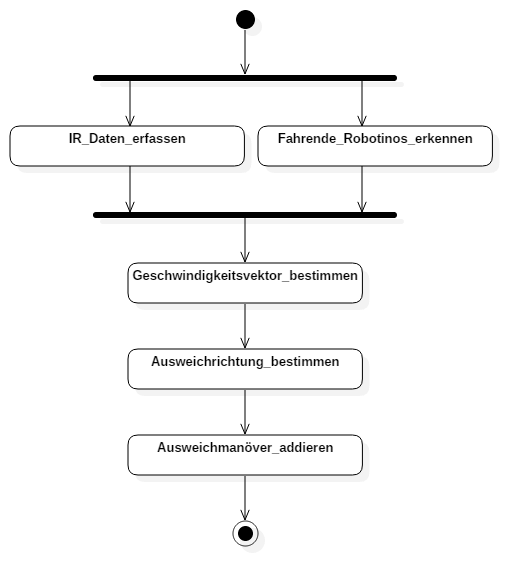
\includegraphics[width=0.5\textwidth]{grafiken/Geschwindigkeit_bestimmen.png}
	\caption{Ablaufplan des Subsystems Vektorberechnung}
	\label{fig:AblVektor}
\end{figure}
Dazu werden zuerst alle ben�tigten Daten bestimmt. Dazu geh�ren die Positionen der bekannten Hindernisse, welche unter Kapitel \ref{sec:bekHindernis} beschrieben sind, und der unbekannten Hindernisse, welche unter Kapitel \ref{sec:unbekHindernis} erl�utert werden. Desweiteren werden die von der Bahnregelung erhaltenen Beobachterdaten als Robotinoposition genutzt, welche in den Formeln die x und y Koordinaten darstellen. Da zuerst die Sollfahrtrichtung bestimmt werden muss, um ein Ausweichman�ver bestimmen zu k�nnen, wird erst der Geschwindigkeitsvektor anhand der Umwelt, des Ziels und der Hindernisse bestimmt. Im n�chsten Schritt wird dann anhand der bekannten Hindernisse ein Ausweichman�ver berechnet, wenn sich ein bekanntes Hindernis in einem Toleranzband in Fahrtrichtung befindet. Im Anschluss wird das Ausweichman�ver auf den Geschwindigkeitsvektor addiert. Bevor der Geschwindigkeitsvektor auf den Sollwerteingang des Robotinos gegeben werden kann, muss der ermittelte Geschwindigkeitsvektor gefiltert und auf lokale Koordinaten transformiert werden.


\section{UDP Gewerk1 einlesen}
In diesem Subsystem wird per UDP alle Daten eingelesen, die an die IP des Robotinos adressiert sind.Der Aufbau des Subsystems ist in Abbildung \ref{fig:UDPGW1} gezeigt Die dabei eingelsesenen Daten wurden unter Kapitel \ref{} n�her erl�utert.
\begin{figure}
	\centering	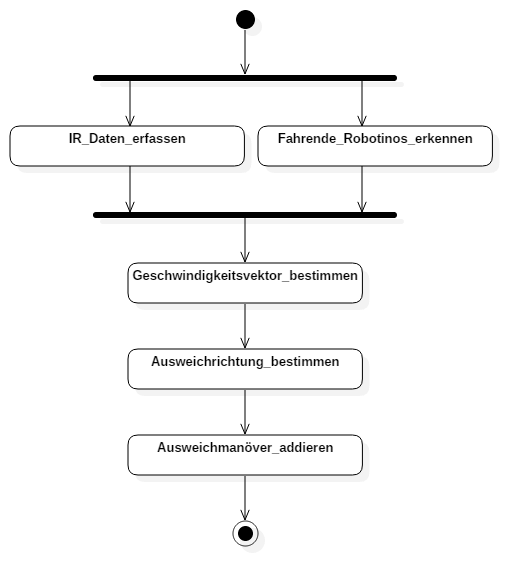
\includegraphics[width=0.5\textwidth]{grafiken/Geschwindigkeit_bestimmen.png}
	\caption{Subsystem UDP Gewerk 1}
	\label{fig:UDPGW1}
\end{figure}

\section{UDP Daten formatieren}
In diesem Subsystem werden die eingelesenen UDP Datenvon der Fertigungsplanung aufgesplittet. Der Aufbau des Subsystems ist in Abbildung \ref{} dargestellt.

\begin{figure}
	\centering	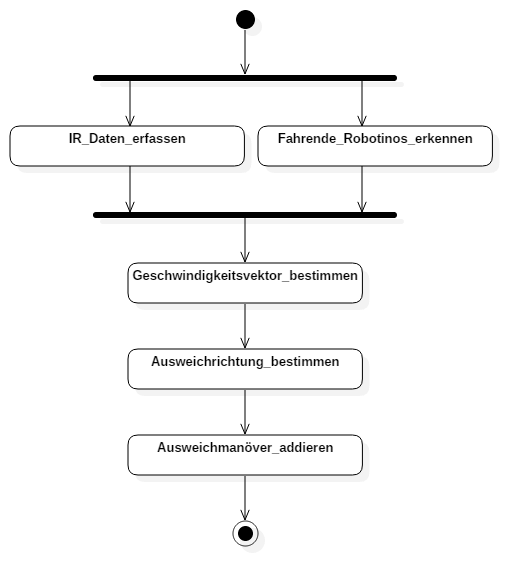
\includegraphics[width=0.5\textwidth]{grafiken/Geschwindigkeit_bestimmen.png}
	\caption{Subsystem Vektorberechnung}
	\label{fig:Vektorberechnung}
\end{figure}

\section{Fehler erkennen}
In dieser Funktion wird sich der Fehlerstatus des Robotinos gemerkt und bei einem Resetsignal durch die Fertigungsplanung zur�ckgesetzt. Desweiteren wird der Fehler erkannt, dass ein Werkst�ck w�hrend des Transport verloren wird, erkannt.

\section{Auftrag steuern}
In diesem Stateflow wird das abarbeiten des Auftrags gesteuert, da wir von der Fertigungsplanung Auftr�ge gesendet bekommen die Startfach und Zielfach enthalten ist dies Notwendig.Das entwickelte Stateflow ist in Abbildung \ref{fig:Auftrag} dargestellt. Dabei ist der Startzustand auf einen neuen Auftrag warten. In diesem Zustand wird der Status auf Frei gesetzt. Wenn nun ein Auftrag eingegangen ist wird unterschieden ob der Robotino laden oder Transportieren soll. Wenn der Robotino Laden soll, wird als Ziel die Ladestation an die folgenden Funktionen �bergeben. Wenn nun ein Signal von der Fertigungsplanung erhalten wird, dass der Robotino fertig geladen hat, wird der Status auf Ladenabgeschlossen gesetzt. Wenn sich nun der Robotino im Transportbereich befindet, also die Ladestation sicher verlassen wurde, wird wider auf einen neuen Auftrag gewartet. Wenn ein Auftrag erhalten wird, der zum Transport dient, wird der Zustand auf Arbeitend ohne Werkst�ck ge�ndert. In diesem Zustand wird als Ziel das Startfach an die nachfolgenden Funktionen �bergeben. Wenn nun ein Werkst�ck aufgenommen ist und sich der Robotino wider im Transportbereich befindet wird der Zusatnd auf Arbeotend mit Werkst�ck gesetzt. In diesem Zustand wird nun das Zielfach als Ziel an die nachfolgenden Funktionen �bergeben. Wenn dann das Werkst�ck abgelegt ist, wird der Zustand auf Werkst�ck abgelegt ge�ndert. Dieser Zustand wird verlassen, wenn der Robotino wider im Transportbereich ist und es kann wider ein neuer Auftrag begonnen werden.

\begin{figure}
	\centering	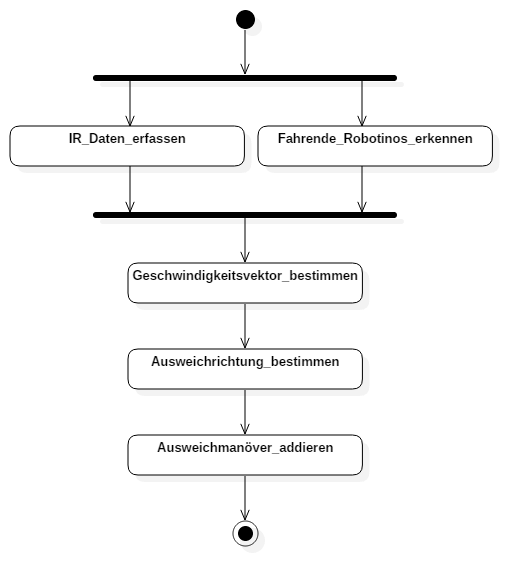
\includegraphics[width=0.5\textwidth]{grafiken/Geschwindigkeit_bestimmen.png}
	\caption{Stateflow Auftrag steuern}
	\label{fig:Auftrag}
\end{figure}


\section{Position der Robotinos bestimmen}
In dieser Funktion wird anhand der RobotinoID und der UDP Daten des Kamerasystems die St�rposition (anderen Robotinos) bestimmt, sowie die eigene Position bestimmt. Da im laufe des Projektes Beobachterdaten durch die Bahnregelung generiert werden, wird die eigene Position nach dieser Funktion mit den Beobachterdaten �berschrieben.

\section{Geschwindigkeit bestimmen}
Um die Sollgeschwindigkeit des Robotinos zu bestimmen, wird das Subsystem Vektorberechnung genutzt. Dieses Subsystem ist wie in Abbildung \ref{fig:Vektorberechnung} dargestellt, aufgebaut. Das Subsystem hat dabei den in Abbildung \ref{fig:AblVektor} gezeigten Ablauf. Dabei ist zu erkennen, dass zuerst die IR Daten erfasst werden und die fahrenden Robotinos erkannt werden. Die IR Datenerfassung wird unter Kapitel \ref{} n�her erl�utert. Wie die fahrenden Robotinos erkannt werden, wird in Kapitel \ref{} beschrieben. Anhand der IR Daten und der Informationen �ber die fahrenden Robotinos wird dann der Geschwindigkeitsvektor bestimmt. Die dabei genutzte Funktion wird unter Kapitel \ref{} beschrieben. Anhand des bestimmten Geschwindigkeitsvektors wird dann eine Ausweichrichtung bestimmt, wenn ein anderer Robotino die Route kreuzt. die dazu genutzte Funktion ist in Kapitel \ref{} n�her beschrieben. Im n�chsten Schritt wird dann das Ausweichman�ver ausgef�hrt. Die Implementierung des Ausweichman�vers wird in Kapitel \ref{} beschrieben.

\begin{figure}
	\centering	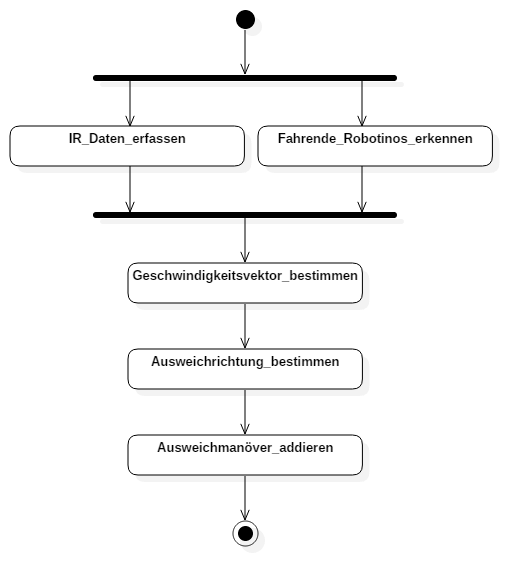
\includegraphics[width=0.5\textwidth]{grafiken/Geschwindigkeit_bestimmen.png}
	\caption{Subsystem Vektorberechnung}
	\label{fig:Vektorberechnung}
\end{figure}

\begin{figure}
	\centering	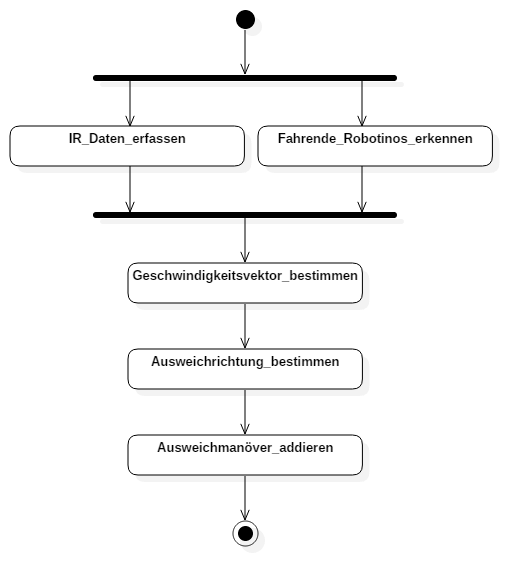
\includegraphics[width=0.5\textwidth]{grafiken/Geschwindigkeit_bestimmen.png}
	\caption{Ablaufplan des Subsystems Vektorberechnung}
	\label{fig:AblVektor}
\end{figure}

\subsection{IR Daten erfassen}
In der IR Daten erfassen Funktion werden zuerst die IR Daten aus den RobotinoDaten gefiltert und auf NaN gesetzt, wenn der gemessene Abstand gr��er als 150 mm ist. Bei einem Abstand kleiner gleich 150 mm wird die Position der Hindernisse in globalen Koordinaten bestimmt und ausgegeben.

\subsection{Fahrende Robotinos erkennen}
Um zu erkennen ob die anderen Robotinos fahren, werden die Postionen der Robotinos mit den Postionen vor einer Sekunde verglichen. Wenn die Robotinos mehr als 10 mm in der Sekunde zur�ckgelegt haben, wird der Robotino als fahrend gesetzt.

\subsection{Geschwindigkeitsvektor bestimmen}
In dieser Funktion wird das in Kapitel \ref{} beschriebene Potentialfeld zur Vektorberechnung umgesetzt. Dazu werden die in Kapitel \ref{} beschriebenen Funktionen abgeleitet und addiert. Die genutzten Ableitungen sind unter \ref{} bis \ref{}dargestellt. Dabei werden die Funktionen partiel nach x und y abgeleitet. In der Funktion \ref{} und \ref{} wird die Ableitung der Stationspotentialfeldes definiert. Diese Funktionen werden im Programm f�r die vier Stationen und die zwei Ladestation ausgef�hrt. Im n�chsten Schritt wird der Zielvektor �ber die abgeleitete Funktion \ref{} und \ref{} bestimmt. Im n�chsten Schritt werden die Robotino und IR Gradienten berechnet. Dazu wird die gleiche Funktion (\ref{} und \ref{}) wie bei der Stationsberechnung genutzt. Dabei werden jedoch die �ber die IR Daten erfassten Positionen, sowie die per Kameraudp erhaltenen Robotinopositionen genutzt. Im n�chsten Schritt wird die aktuelle Robotinozone bestimmt und je nach Zone der Umweltgradient, nach den Funktionen \ref{} bis \ref{}, bestimmt. Da nicht alle Gradienten in allen Zonen genutzt werden, gibt es jeder Zone eine eigene Summe von Gradienten. Dabei wird zum Beispiel die Stationsgradienten der Stationen nur in Zone 4 und die Ladestationsgradienten nur in Zone 0 mit eingerechnet. Desweiteren wird der Zielgradienten nur in Zone 0 eingerechnet damit die F�hrung des Robotinos hinter den Statonen nicht gest�rt wird.

\begin{align}
Vx_{Stationen}=-K\cdot e^{-\frac{(x-Stationsposition_x)^2+(y-Stationsposition_y)^2}{2\cdot \sigma^2}} \cdot \frac{x-Stationsposition_x}{2\cdot \sigma^2}\\
Vy_{Stationen}=-K\cdot e^{-\frac{(x-Stationsposition_x)^2+(y-Stationsposition_y)^2}{2\cdot \sigma^2}} \cdot \frac{y-Stationsposition_y}{2\cdot \sigma^2}\\
Vx_{Ziel}=\frac{K\cdot(x-Ziel_x)}{\sqrt{(x-Ziel_x)^2+(y-Ziel_y)^2}}\\
Vy_{Ziel}=\frac{K\cdot(y-Ziel_y)}{\sqrt{(x-Ziel_x)^2+(y-Ziel_y)^2}}\\
Vx_{Umwelt}(Zone=0,x=0..5500,y=0..2500)=\frac{1}{\sigma}\cdot K \cdot e^{\frac{-x}{\sigma}} +\frac{-1}{\sigma}\cdot K \cdot e^{\frac{x-x_{max}}{\sigma}}\\
Vy_{Umwelt}(Zone=0,x=0..5500,y=0..2500)=\frac{-1}{\sigma} \cdot K \cdot e^{\frac{y-2500}{\sigma}} +\frac{1}{\sigma} \cdot K \cdot e^{\frac{-y}{\sigma}}\\
Vx_{Umwelt}(Zone=0,x=5500..x_{max},y=0..2500)=\frac{1}{\sigma}\cdot K \cdot e^{\frac{-(x-5500)+(y-2500)}{\sigma}} +\frac{-1}{\sigma}\cdot K \cdot e^{\frac{x-x_{max}}{\sigma}}\\
Vy_{Umwelt}(Zone=0,x=5500..x_{max},y=0..2500)=\frac{-1}{\sigma} \cdot K \cdot e^{\frac{-(x-5500)+(y-2500)}{\sigma}} +\frac{1}{\sigma} \cdot K \cdot e^{\frac{-y}{\sigma}}\\
Vx_{Umwelt}(Zone=0,x=5500..x_{max},y=2500..y_max)=\frac{1}{\sigma}\cdot K \cdot e^{-\frac{x-5500}{\sigma}} +\frac{-1}{\sigma}\cdot K \cdot e^{\frac{x-x_{max}}{\sigma}}\\
Vy_{Umwelt}(Zone=0,x=5500..x_{max},y=2500..y_{max})=\frac{-1}{\sigma} \cdot K \cdot e^{\frac{y-y_{max}}{\sigma}} +\frac{1}{\sigma} \cdot K \cdot e^{\frac{-y}{\sigma}}\\
Vx_{Umwelt}(Zone=1)=K_{gerade}\\
Vy_{Umwelt}(Zone=1)=-2\cdot \frac{y-3500}{K_{parabel}}\\
Vx_{Umwelt}(Zone=2)=-K_{gerade}\\
Vy_{Umwelt}(Zone=2)=-2\cdot \frac{y-3500}{K_{parabel}}\\
Vx_{Umwelt}(Zone=3)=-2\cdot \frac{x-300}{K_{parabel}}\\
Vy_{Umwelt}(Zone=3)=-K_{gerade}\\
Vx_{Umwelt}(Zone=4)=0\\
Vy_{Umwelt}(Zone=4)=K_{gerade}\\
Vx_{Umwelt}(Zone=5)=-2\cdot \frac{x-5500}{K_{parabel}}\\
Vy_{Umwelt}(Zone=5)=-K_{gerade}
 \end{align}

\subsection{Ausweichrichtung bestimmen}
Um eine Ausweichrichtung zu bestimmen, wird zuerst der Abstand zu den anderen Robotinos anhand derer Positionen bestimmt. Wenn der Abstand geringer als ein Meter ist, wird der globale Winkel zum Robotino bestimmt und um \(90^�\) erh�ht. Zus�tzlich wird im n�chsten Schritt der Fahrwinkel anhand des Geschwindigkeitsvektors in globalen Koordinaten bestimmt. Anhand des Fahrwinkels und der Robotinowinkel wird dann ein Enable-Bit gesetzt wenn sich der Robotino in einem Toleranzbereich um den Fahrwinkel befindet. Wenn dieses Enable-Bit nicht gesetzt ist, wird kein Ausweichman�ver ausgef�hrt.

\subsection{Ausweichman�ver addieren}
In dieserFunktion wird nun auf das Ausweichman�ver auf den Geschwindigkeitsvektor addiert wenn das Enable-Bit aus der Ausweichrichtungsbestimmung gesetzt ist. Desweiteren wird das Ausweichman�ver nicht ausgef�hrt wenn sich der Robotino nicht in der Hauptfahrzone (Zone=0) befindet oder sich der Robotino nicht im FIFO-Bereich oder nahe am Ziel (Distanz >300mm) befindet.
Zus�tzlich wird in dieser Funktion die Abbremsfilterung integriert, wie im Kapitel \ref{} beschrieben, wird dazu ein distanzabh�ngiger Faktor multipliziert.

\section{Fahrmodus steuern}
Diese Stateflow, welches in Abbildung \ref{fig:Fahrmodus} dargestellt ist, steuert die Kommunikation mit der Bahnregelungsgruppe. Beim Start ist der Transportbereich aktiv in dem die Potentialfeldmethode zum Regeln genutzt wird. Wenn der Robotino �ber das Potentialfeld sein Ziel erreicht hat, wird an die Bahnregelung, �ber das setzen des Fertigungsbereich auf eins, �bergeben. Wenn das Ziel eine Ladestation ist, wird der Bahnregelung die Zielladestationsposition �bergeben. Wenn der Robotino fertig geladen hat, wird der Bahnregelung wieder der �bergabepunkt als Ziel gegeben und wieder auf den Transportbereich gewechselt.\\
Wenn das Ziel eine Ladestation ist werden zwei varianten unterschieden. Die erste M�glichkeit besteht darin ein Werkst�ck aufzunehmen. Dabei wird zuerst die Werkstueckposition �bergeben. Nach der Best�tigung von der Bahnregelung des erfolgreichen aufnehmens, wird der RFID-Leser als Ziel vorgegeben. Wenn die Bahnregelung die Position best�tigt, wird auf eine Best�tigung, desRFID-Schreibens, durch die Fertigungsplannung gewartet. Nach dieser Best�tgung wird der Bahnregelung ein �bergabepunkt vorgegeben an dem zur Potentialfeldmethode gewechselt werden soll. Dabei besteht die M�glichkeit nach hinten abzugeben, wenn ein Robotino auf die Station wartet oder nach vorne abzugeben wenn kein Robotino in die Station m�chte.\\
Im zweiten Fall soll ein Werkst�ck in der Station abgegeben werden. Dabei �ndert sich Reihenfolge der Ziele auf als erstes zum RFID-Leser und auf best�tigung von Fertigungsplanung warten. Als n�chstes die Zielposition f�r das Werkst�ck und wieder die Ausfahrposition.\\
In diesem Stateflow erfolgt zus�tzlich die Statuszuweisung des Robotinos und dessen Fehlererkennung.

\begin{figure}
	\centering	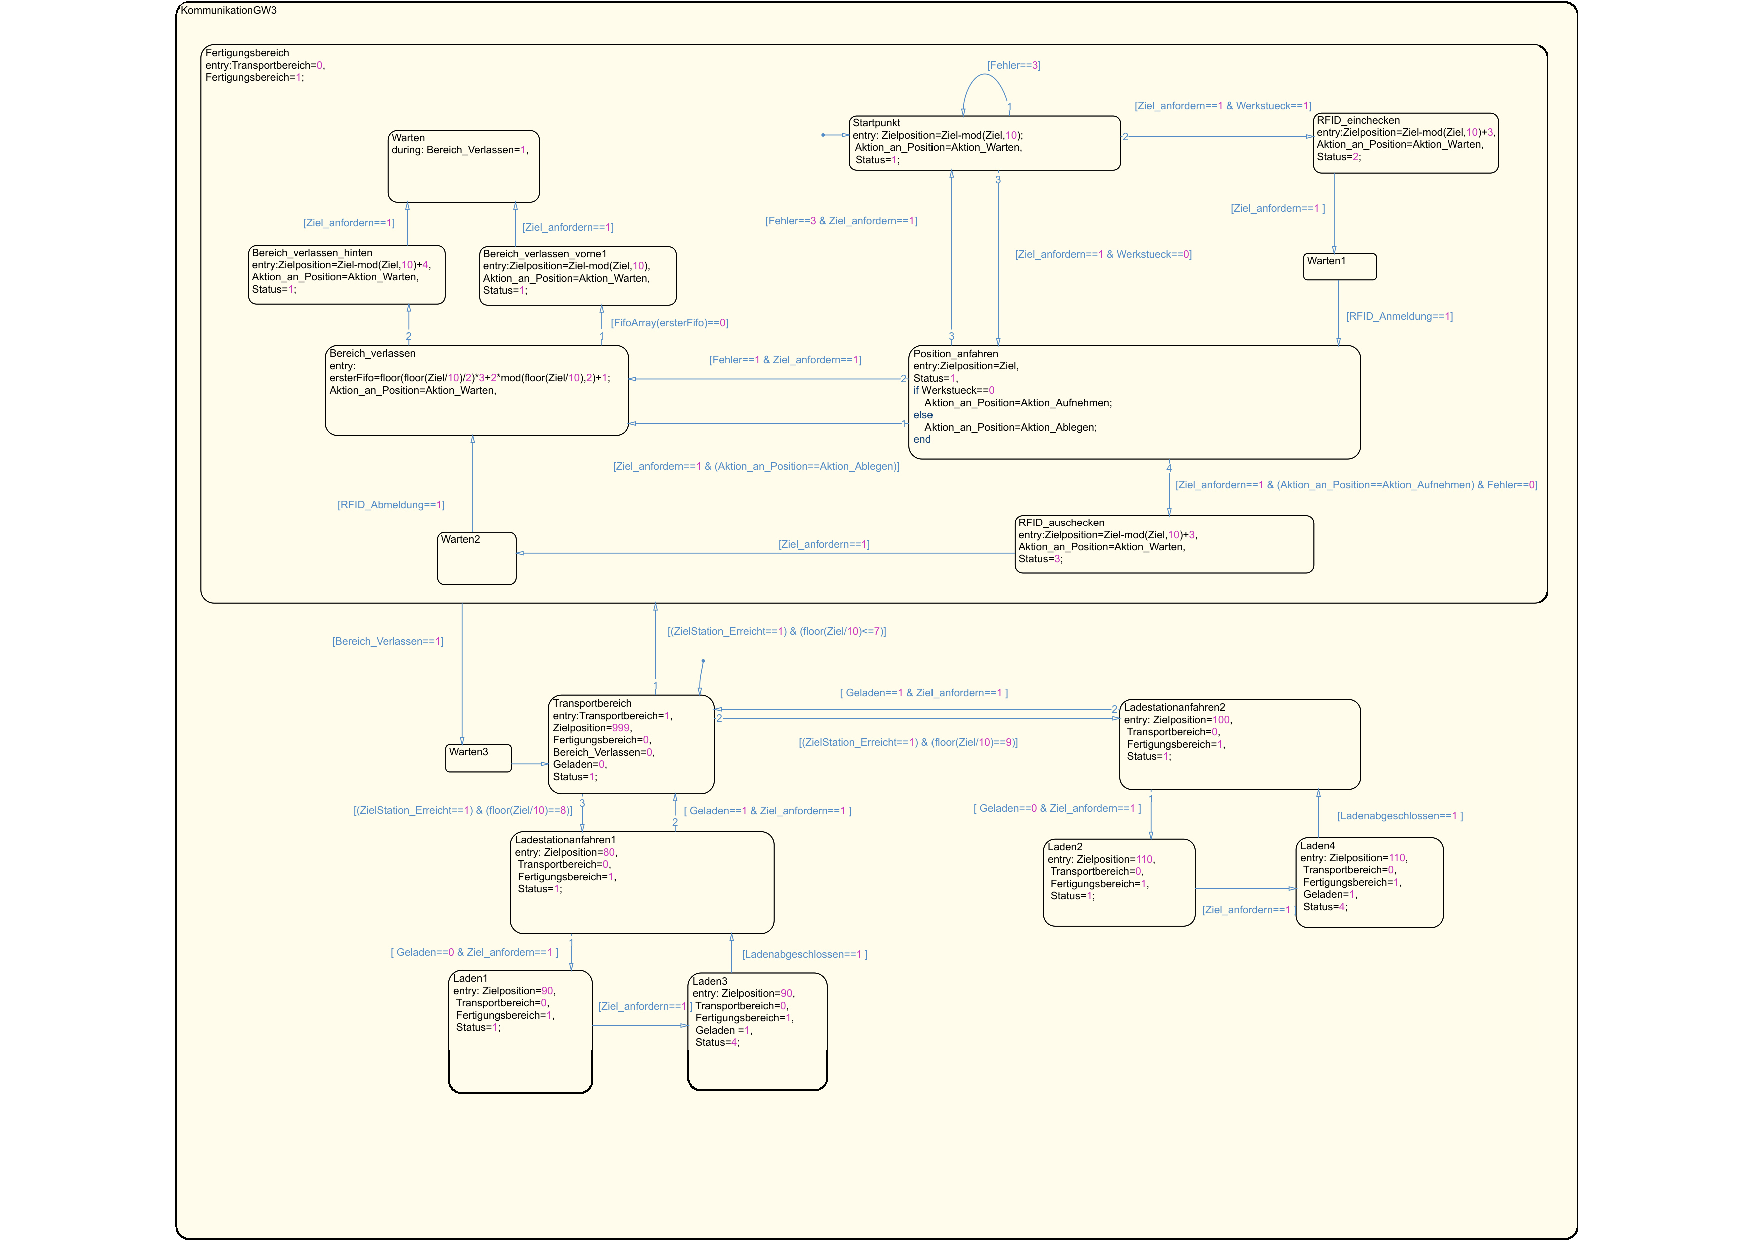
\includegraphics[width=1\textwidth]{grafiken/KommunikationGewerk3.pdf}
	\caption{Fahrmodus steuern}
	\label{fig:Fahrmodus}
\end{figure}

\section{Geschwindigkeit begrenzen}
In dieser Funktion wird eine gleitende Mittelwertbildung �ber 100 Werte vorgenommen um die Geschwindigkeitsvorgabe zu gl�tten.  Nach der Filterung wird die Geschwindigkeit je nach Position begrenzt. Dabei wird die Geschwindigkeit bei den FIFO-Positionen auf 300mm/s begrenzt und in der Hauptfahrzone auf 700mm/s.

\section{Geschwindigkeit transformieren}
In dieser Funktion wird der globale Geschwindigkeitsvektor auf das Robotinokoordinatensystem �ber den Winkel des Robotinos transformiert. Dazu wird eine Rotationsmatrix genutzt. Da der Robotino den negativen Gradienten in mm/s als vorgabe ben�tigt, wird der Geschwindigkeitsvektor vor diesem Funktionblock mit -1000 multipliziert, da durch unsere Berechnung der positive Gradent in m/s ermittelt wird.

\section{Status bestimmen}
In dieser Funktion wird der Status des Robotinos, der an die Fertigungsplanung �bergeben wird, bestimmt. Dabei wird der Status der in der Fahrmodussteuerung unter Kaptel \ref{} direkt �bergeben wenn kein Fehler durch die Bahnregelung registriert wird.

\section{UDP Gewerk1 schreiben}
In diesem Subsystem wird die UDP-Kommunikation mit der Fertigungsplanung realisiert, dazu werden die zu sendenden Daten gepackt und per UDP an alle im Netzwerk geschickt. Der Aufbau des Subsystems ist in Abbildung \ref{} unter Kapitel \ref{} gezeigt. Dazu wird f�r jeden Robotino ein eigener Port definiert.Die Schnittstelle unter Kapitel \ref{} n�her erl�utert.







%\chapter{Robotino 2.0}
\chapter{Robotino 2.0}\label{cha:Robo2.0}
In diesem Kapitel wird beschrieben, welche Anpassungen am Programm vorgenommen werden m�ssen, um das Programm von den alten Robotinos auf dem neuen Robotino lauff�hig zu bekommen. Um das Programm auf den Robotino 2.0 anzupassen, wird eng mit der Bahnregelung und Gewerk4 zusammengearbeitet. In Absprache mit der Bahnregelung wird eine Anpassung der Ladestationsanfahrpositionen vorgenommen, da der Robotino 2.0 die Ladestation anders anfahren muss als die alten Robotinos. Da f�r den Robotino 2.0 ein anderes Starterkit ben�tigt wird, wird Gewerk�bergreifend ein Robotino 2.0 Starterkit erstellt. Da diese �nderungen am Starterkit im Bahnplanungsblock nur Einfluss auf die UDP Kommunikation mit der Auftragssteuerung hat, wird der Simulinkblock zur UDP-Kommunikation durch ein Output und Input in den gesamt Bahnplanungsblock ersetzen. Da die UDP-Kommunikationsblock von Simulink nicht in Twincat ausgef�hrt werden kann, m�ssen die per Input und Ouput definierten UDP Daten auf den in Twincat integrierten UDP-Kontroller gemappt werden. Da auf dem Robotino 2.0 zu Programmstart die Zielposition und die Robotinoposition auf [0 0 0] gesetzt ist, muss im Programm eine Division durch 0 bei Programmstart vermieden werden, da im Zielpotentialfeld in diesem Fall durch 0 dividiert wird. Dieses Problem wird durch eine if Abfrage behoben, indem der Zielvektor auf 0 gesetzt wird, wenn die Robotinoposition gleich der Zielposition ist.
\chapter{Validierung}
%\chapter{Ausblick}
%\chapter{Fazit}






